\documentclass[
  ngerman,
  a4paper,
  12pt
]{report}

\newcommand{\keypub}{k_{pub}}
\newcommand{\keypr}{k_{pr}}

\usepackage[utf8]{inputenc}
\usepackage[german]{babel}
\usepackage[left=2.5cm, right=2.5cm]{geometry}
\usepackage{csquotes}
\usepackage{setspace}
\usepackage[dvipsnames]{xcolor}
\usepackage{caption} % http://ftp.rrzn.uni-hannover.de/pub/mirror/tex-archive/macros/latex/contrib/caption/caption-eng.pdf

\usepackage{graphicx}
\graphicspath{{./images}}

\usepackage[boxruled, algochapter, longend]{algorithm2e} % http://ftp.rrzn.uni-hannover.de/pub/mirror/tex-archive/macros/latex/contrib/algorithm2e/doc/algorithm2e.pdf
\SetAlgoCaptionLayout{centerline}
\SetKw{GoTo}{goto}
\SetKwProg{Marker}{}{:}{}

\usepackage{enumitem}
\setlist{itemsep=0pt}

\usepackage{hyperref}
\hypersetup{
  colorlinks = true,
  linkcolor = Red,
  filecolor = Magenta,      
  urlcolor = Green,
  citecolor = Cyan
}

\usepackage[shortcuts]{glossaries}
\makenoidxglossaries
\newacronym{des}{DES}{Data Encryption Standard}
\newacronym{aes}{AES}{Advanced Encryption Standard}
\newacronym{rng}{RNG}{\textit{random number generator}}
\newacronym{trng}{TRNG}{\textit{true random number generator}}
\newacronym{prng}{PRNG}{\textit{pseudo random number generator}}
\newacronym{csprng}{CSPRNG}{\textit{cryptographically secure pseudo random number generator}}
\newacronym{otp}{OTP}{One-Time-Pad}
\newacronym{lsb}{LSB}{\textit{least significant bit}}
\newacronym{jwt}{JWT}{JSON Web Token}

\usepackage[style = authoryear-ibid]{biblatex}
\addbibresource{others/main.bib}

\usepackage{tikz}
\usetikzlibrary{positioning, calc, arrows, shapes}
\tikzset{>=triangle 45}
% https://tex.stackexchange.com/questions/75836/creating-a-seamless-xor-symbol-as-node
\tikzset{XOR/.style={draw,circle,append after command={
          [shorten >=\pgflinewidth, shorten <=\pgflinewidth,]
          (\tikzlastnode.north) edge (\tikzlastnode.south)
          (\tikzlastnode.east) edge (\tikzlastnode.west)
        }
    }
}
\tikzset{unsecure channel/.style={draw, align=center, inner xsep=-0.1cm, inner ysep=0.3cm, ellipse}}

\usepackage{amssymb}
\usepackage{amsmath}
\usepackage{amsthm}
\theoremstyle{plain}
\newtheorem{lemma}{Lemma}[section]
\newtheorem{satz}{Satz}[section]
\newcommand{\satzautorefname}{Satz}

\theoremstyle{definition}
\newtheorem{definition}{Definition}[section]
% https://tex.stackexchange.com/questions/16453/denoting-the-end-of-example-remark
\newtheorem{examplex}{\normalfont\textit Beispiel}[section]
\newenvironment{example}
  {\pushQED{\qed}\renewcommand{\qedsymbol}{$\triangle$}\examplex}
  {\popQED\endexamplex}

\theoremstyle{remark}
\newtheorem{remark}{Bemerkung}[section]

\newcommand{\ggt}[2]{ggT(#1,#2)}
\newcommand{\numeq}[1]{\stackrel{#1}{=}}
\newcommand{\phif}[1]{\ensuremath{\varphi(#1)}}

\begin{document}
\pagenumbering{Roman}
\newcommand{\DhbwLogo}{
\includegraphics[width=4cm]{dhbw-logo.png}}
\newcommand{\Titel}{Grundlagen der Kryptografie und Steganografie}
\newcommand{\Was}{Studienarbeit}
\newcommand{\Abschluss}{Bachelor of Science}
\newcommand{\Studiengang}{Informatik / Angewandte Informatik}
\newcommand{\Author}{\textbf{Jens Döllmann}}
\newcommand{\Abgabedatum}{17. Mai 2021}

\newcommand{\Dauer}{2 Semester}
\newcommand{\Matrikelnummer}{8876462}
\newcommand{\Kursbezeichnung}{TINF18B4}
\newcommand{\FirmenName}{Siemens AG}
\newcommand{\FirmenStadt}{Karlsruhe}
\newcommand{\BetreuerFirma}{Florian Seiter}
\newcommand{\BetreuerDHBW}{Ralf Brune}

% Titelseite
\begin{titlepage}
  \vspace*{-2cm}
  \DhbwLogo
  \vspace{1cm}
  \begin{center}
    \huge
    \Titel\\[1cm]
    {\scshape \Was}\\[1cm]
    \large
    für die Prüfung zum\\[0.5cm]
    \Abschluss\\[0.5cm]
    des Studiengangs \Studiengang\\[0.5cm]
    an der\\[0.5cm]
    Dualen Hochschule Baden-Württemberg Karlsruhe\\[0.5cm]
    von\\[0.5cm]
    \Author\\[1cm]
    Abgabedatum \Abgabedatum
  \end{center}

  \vfill

  \begin{tabular}{l@{ \hspace{2cm} }l}
    Bearbeitungszeitraum          & \Dauer           \\
    Matrikelnummer                & \Matrikelnummer  \\
    Kurs                          & \Kursbezeichnung \\
    Gutachter der Studienakademie & \BetreuerDHBW    \\
  \end{tabular}
\end{titlepage}

\onehalfspacing

% Verzeichnisse 
\tableofcontents
\listoftables
\listoffigures
\listofalgorithms

% Kapitel
\newpage
\pagenumbering{arabic}
\chapter{Einleitung} \label{cha:einleitung}
Redet man heutzutage über das Thema Kryptografie, sind im Gespräch wahrscheinlich
Themen wie E-Mail-Verschlüsselung, Internetprotokolle oder Anwendungen im
Bankenwesen. Auch bekannt sind die Angriffe auf kryptografische Systeme
wie die Entzifferung der durch die Enigma-Chiffriermaschine
verschlüsselten deutschen Funksprüche während des Zweiten Weltkrieges. Es scheint, als
wäre Kryptografie stark mit den modernen elektronischen Kommunikationstechniken
verbunden. Dies ist allerdings nicht so: Frühe Formen der Kryptografie
gehen zurück bis etwa 2000 v.\,Chr., als bereits im antiken Ägypten neben den
Standard-Hieroglyphen zusätzlich auch \enquote{geheime} Zeichen
verwendet wurden \parencite[2]{BOOK:crypto}. Es werden prinzipiell zwei
Varianten kryptografischer Verfahren unterschieden, diese sind
symmetrische und asymmetrische Algorithmen. Die symmetrische Verschlüsselung ist
seit langer Zeit ein fester Bestandteil der Kryptografie mit bekannten historischen
Verfahren wie die Cäsar-Chiffre, welche bereits im antiken Rom für das Verschlüsseln von
Nachrichten verwendet wurde. Asymmetrische Verschlüsselung hingegen ist eine gänzlich neue Form
der Kryptografie, Whitfield Diffie, Martin Hellman und Ralph Merkle haben die Idee im Jahr
1976 erstmalig öffentlich eingeführt \parencite[3]{BOOK:crypto}.
Eine Übersicht über das Gebiet der Kryptografie ist in \autoref{fig:kryptologie} zu sehen.
Es ist zu bemerken, dass an oberster Stelle nicht die Kryptografie, sondern
der Oberbegriff Kryptologie zu finden ist, welche sich in die drei großen Bereiche unterteilt:

\begin{figure}
  \centering
  \begin{tikzpicture}
    [every node/.style={draw, inner xsep=4mm, inner ysep=2mm, rounded corners=2mm, align=center}]
    \node(root) {Kryptologie};

    \node [below= of root] (analyse) {Kryptanalyse};
    \node [left= of analyse] (crypto) {Kryptografie};
    \node [right= of analyse, dashed] (stego) {Steganografie};

    \node [below left= of crypto] (sym) {Symmetrische \\ Chiffren};
    \node [below= of crypto] (asym) {Asymmetrische \\ Chiffren};
    \node [below right= of crypto] (prot) {Protokolle};

    \coordinate (x) at ($(root.south) - (0, 0.5cm)$);
    \draw (root) -- (x);
    \draw [->] (x) -| (stego);
    \draw [->] (x) -| (crypto);
    \draw [->] (x) -| (analyse);

    \coordinate (y) at ($(crypto.south) - (0, 0.5cm)$);
    \draw (crypto) -- (y);
    \draw [->] (y) -| (sym);
    \draw [->] (y) -| (asym);
    \draw [->] (y) -| (prot);
  \end{tikzpicture}

  \caption{Die Kryptologie und ihre Untergebiete \parencite[3]{BOOK:crypto}}
  \label{fig:kryptologie}
\end{figure}

\paragraph{Kryptografie}
Die Wissenschaft, eine Nachricht so zu verändern, dass ihr Sinn nur von dem Empfänger
verstanden werden kann, für den sie bestimmt ist.

\paragraph{Kryptanalyse}
Die Wissenschaft, ein kryptografisches System zu analysieren mit dem Ziel, mögliche
Schwachstellen aufzudecken. Die Kryptanalyse ist ein äußerst wichtiger Teil der
Kryptologie, denn ohne Personen, welche versuchen ein kryptografisches System zu
brechen, wird man nie herausfinden können, ob dieses wirklich sicher ist.

\paragraph{Steganografie}
Die Kunst, Informationen in einer für den Computer
zugänglichen Trä\-gerdatei (engl. \textit{cover media}) zu verstecken, sodass eine
weitere Person die Existenz einer geheimen Botschaft gar nicht erst vermuten würde.
Die Steganografie wird in der Literatur häufig nicht als ein Bereich der Kryptologie
erwähnt, soll aber als wesentlicher Teil dieser Studienarbeit auch hier
schon betrachtet werden. Es ist wichtig abzugrenzen, dass es sich
im Gegensatz zu den Chiffren der Kryptografie nicht um ein Verschlüsselungsverfahren handelt
und ein Außenstehender, welcher von der Existenz einer geheimen Nachricht Bescheid weiß,
diese unverschlüsselt lesen könnte.\\[8pt]
Ein starkes Kryptoverfahren sollte dem \textit{Kerckhoffs's principle} unterliegen, welches
im Jahr 1883 von Auguste Kerckhoffs postuliert wurde und von \citeauthor{BOOK:crypto}
durch folgende Definition beschrieben ist \parencite*[11]{BOOK:crypto}:

\begin{definition}[\textit{Kerckhoffs's principle}]
  \enquote{\textit{A cryptosystem should be secure even if the attacker knows all details about
      the system, with the exception of the secret key. In particular, the system should be secure when
      the attacker knows the encryption and decryption algorithms.}}
\end{definition}

\noindent
Auf den ersten Blick scheint das \textit{Kerckhoffs's principle} nicht sonderlich intuitiv.
Es sei einfach zu glauben, dass ein System
sicherer sein muss, wenn die Details der Implementierung geheim gehalten werden.
In der Regel ist dies aber nicht so. Ein Kryptoverfahren bleibt nicht für immer geheim und die
Vergangenheit hat gezeigt, dass ein System, dessen geheimes Design an die Öffentlichkeit
gelangt, fast immer unsicher ist. Ein hierfür gutes Beispiel ist das Content Scrambling System (CSS)
für das Verschlüsseln von DVD-Videoinhalten. Trotz großer Bemühungen der Industrie, die
Funktionsweise von CSS geheim zu halten, gelang das Design durch Reverse Code Engineering
schnell an die Öffentlichkeit. Es zeigten sich Mängel in der Implementierung,
welche das Brechen der Verschlüsselung mit sehr geringen Aufwand ermöglichten \parencite{SITE:CSS}.
Am Beispiel von symmetrischen und asymmetrischen Verschlüsselungsverfahren werden in den
folgenden Kapiteln Begriffe und Ideen aus dem Bereich der Kryptografie eingeführt.
Zusätzlich wird in \autoref{cha:steganografie} gezielt darauf eingegangen,
wie ein steganografischer Algorithmus entworfen werden kann.
Der Algorithmus soll eine beliebig lange Nachricht in einer Bilddatei verstecken,
ohne dabei die visuelle Qualität sichtbar zu beeinflussen. Es werden Fragen untersucht,
wie stark ein Bild angepasst werden kann und ab welcher Nachrichtenlängen
eine Veränderung sichtbar wird.
\section{Symmetrische Verschlüsselung}
Denkt man an die Teilbereiche der Kryptografie, ist die symmetrische Verschlüsselung
das wohl klassischste Beispiel. Zwei Parteien kommunizieren mit einem
Algorithmus zum Ver- und Entschlüsseln von Nachrichten und haben sich auf einen
gemeinsamen geheimen Schlüssel geeinigt. Wie es in der Literatur sehr beliebt ist,
wird die Idee der symmetrischen Verschlüsselung
mit einem einfachen Beispiel eingeführt \parencite[4-6]{BOOK:crypto}:
Zwei Parteien Alice und Bob möchten über einen unsicheren Kanal Nachrichten untereinander austauschen.
Ein unsicherer Kanal ist hierbei lediglich die Kommunikationsstrecke,
z.\,B. das Internet, die Luftschnittstelle bei WLAN und Mobilfunk
oder jedes andere Medium, über das sich digitale Daten übertragen lassen.
\newpage

\begin{figure}[h]
  \centering

  \begin{tikzpicture}
    [box/.style={draw, align=center},
      rounded/.style={rounded corners=2mm}]

    \node[box, inner xsep=-0.1cm, inner ysep=0.3cm, ellipse]
    (K) {\small unsicherer Kanal \\ \small (z.B. Internet)};
    \node[left=3cm of K, box, rounded] (A) {\small Alice};
    \node[right=3cm of K, box, rounded] (B) {\small Bob};
    \node[above=of K, box, rounded] (O) {\small Oscar \\ \small (Angreifer)};

    \draw[->] (A) -- node[near start, above] {\small $x$} (K);
    \draw[->] (K) -- node[right] {\small $x$} (O);
    \draw[->] (K) -- node[near end, above] {\small $x$} (B);
  \end{tikzpicture}

  \caption{Kommunikation über einen unsicheren Kanal}
\end{figure}

\noindent
Es ist klar, warum Alice und Bob gerne geheime Nachrichten austauschen würden: Alice möchte sich an ihrem
Bankkonto anmelden und sendet ihr Passwort zu Bob. Ein potenzieller Angreifer Oscar
soll die Passwörter von Alice nicht in Klartext mitlesen können.
In einer solchen Situation bietet die symmetrische Verschlüsselung eine gute Lösung:
Bevor Alice ihr Passwort sendet, verschlüsselt sie es mit einem symmetrischen Algorithmus.
Bob invertiert die Verschlüsselung und erhält die unverschlüsselte Nachricht. Wurde für
die Verschlüsselung ein sicherer Algorithmus gewählt, erscheint die Nachricht für Oscar nur wie
eine zufällige Folge von Bit.

\begin{figure}[h]
  \centering

  \begin{tikzpicture}
    [box/.style={draw, align=center},
      rounded/.style={rounded corners=2mm}]

    \node[unsecure channel]
    (K) {\small unsicherer Kanal \\ \small (z.B. Internet)};

    \node[left=of K, box] (E) {\small Verschlüsselung \\ \small $e(x)$};
    \node[left=of E, box, rounded] (A) {\small Alice};

    \node[right=of K, box] (D) {\small Entschlüsselung \\ \small $d(y)$};
    \node[right=of D, box, rounded] (B) {\small Bob};

    \node[above=of K, box, rounded] (O) {\small Oscar \\ \small (Angreifer)};

    \node[below=of K, cylinder, draw, shape border rotate=180] (SK) {\small sicherer Kanal};

    \draw[->] (A) -- node[above] {\small $x$} (E);
    \draw[->] (E) -- node[above] {\small $y$} (K);

    \draw[<-] (B) -- node[above] {\small $x$} (D);
    \draw[<-] (D) -- node[above] {\small $y$} (K);

    \draw[<-] (O) -- node[right] {\small $y$} (K);

    \draw[->] ($(SK.top) + (2.5mm, 0)$) -| node[near end, right] {\small $k$} (E.south);
    \draw[->] (SK) -| node[near end, right] {\small $k$} (D.south);
  \end{tikzpicture}

  \caption{Kommunikation mit symmetrischer Verschlüsselung}
  \label{fig:sym-encryption}
\end{figure}

\noindent
Die Variablen $x, y$ und $k$ aus \autoref{fig:sym-encryption} haben in der
Kryptografie eine besondere Bedeutung:

\begin{itemize}
  \item $x$ ist der Klartext (engl. \textit{plaintext}).
  \item $y$ ist das Chiffrat oder der Geheimtext (engl. \textit{ciphertext}).
  \item $k$ ist der Schlüssel (engl. \textit{key}).
  \item $e$ bezeichnet die Verschlüsselung (engl. \textit{encryption}).
  \item $d$ bezeichnet die Entschlüsselung (engl. \textit{decryption}),
        d.\,h. die Umkehrung von $e$.
\end{itemize}

\noindent
Für die symmetrische Verschlüsselung wird der geheime Schlüssel $k$ benötigt. Dieser
muss vor der Kommunikation auf einem sicheren Weg zwischen Alice und Bob verteilt werden.

\section{Modulare Arithmetik}
Fast alle kryptografischen Algorithmen, sowohl symmetrische als auch asymmetrische Chiffren
basieren auf Arithmetik in einer endlichen Menge von ganzen Zahlen \parencite[13]{BOOK:crypto}.
Dies steht im Gegensatz zu der Mathematik (und dem Alltagsleben),
in der wir es gewohnt sind, in unendlichen
Mengen zu rechnen, z.\,B. den natürlichen oder den reellen Zahlen. Die modulare Arithmetik,
d.\,h. die Division mit Rest bietet eine gute Möglichkeit, um mit diesen begrenzten Mengen
zu arbeiten.

\begin{lemma}[{\cite[179-180]{BOOK:numberTheory}}]
  Folgende Aussagen über drei ganze Zahlen $a$, $b$, $m$, wobei $m > 0$, sind äquivalent:
  \begin{enumerate}[label=\roman*)]
    \item $a$ und $b$ lassen bei Division mit Rest durch $m$ denselben Rest.
    \item Die Differenz $a - b$ ist durch $m$ teilbar.
  \end{enumerate}
\end{lemma}
\begin{proof}
  Es seien $a = q_1m + r_1$ und $b = q_2m + r_2$ mit $0 \leq r_1,r_2 < m$
  und  $q_1,q_2,r_1,r_2 \in \mathbb{Z}$, die Gleichungen,
  die bei Division mit Rest entstehen. \\
  \textit{i)} $\Rightarrow$ \textit{ii)}: \\
  Es gilt: $r_1 = r_2$. \\
  Zu zeigen: $m \mid (a-b)$.
  \begin{align*}
    a - b & = q_1m + r_1 - q_2m - r_2    \\
    a - b & = (q_1 - q_2)m + (r_1 - r_2) \\
    a - b & = (q_1 - q_2)m
  \end{align*}
  Aus der letzten Gleichung folgt: $m \mid (a - b)$. \\
  \textit{ii)} $\Rightarrow$ \textit{i)}: \\
  Es gilt: $m \mid (a - b)$. \\
  Zu zeigen: $r_1 = r_2$.
  \begin{align*}
    m                 & \mid (a - b)                    \\
    \Leftrightarrow m & \mid (q_1 - q_2)m + (r_1 - r_2)
  \end{align*}
  Teilt $m$ zwei Zahlen $a$ und $b$, muss $m$ auch eine Linearkombination dieser Zahlen teilen.
  \begin{align*}
    m                 & \mid (q_1 - q_2)m + (r_1 - r_2) \wedge m \mid (q_1 - q_2)m \\
    \Rightarrow m     & \mid (q_1 - q_2)m + (r_1 - r_2) - (q_1 - q_2)m             \\
    \Leftrightarrow m & \mid (r_1 - r_2)
  \end{align*}
  Aus der letzten Zeile folgt wegen $0 \leq r_1,r_2 < m$ sofort $r_1 - r_2 = 0$.
  Es folgt: $r_1 = r_2$.
\end{proof}

\noindent
Nach Gauß nennt nennt man zwei Zahlen $a, b \in \mathbb{Z}$, die bei der Division durch $m$
denselben Rest ergeben, \textit{kongruent Modulo m}. Anstelle der schwerfälligen
Teilbarkeitsschreibweise $m \mid (a - b)$
führte Gauß folgende Schreibweise ein \parencite[180]{BOOK:numberTheory}:
\begin{equation}
  \label{eq:kongruenz}
  a \equiv b \pmod{m} \text{\quad oder kürzer:\quad} a \equiv b \pod{m}
\end{equation}

\begin{example}
  Es sind $a = 29$ und $m = 8$. Man schreibt
  \begin{equation*}
    29 \equiv 5 \pmod{8} \text{\quad oder als Gleichung:\quad} 29 = 3 \cdot 8 + 5
  \end{equation*}
  und deshalb $8 \mid (29 - 5)$.
\end{example}

\noindent
\autoref{eq:kongruenz} hat unendlich viele Lösungen.
Elemente welche bei Division durch $m$ denselben Rest ergeben,
können in eine Klasse zusammengefasst werden, diese nennt man dann eine Restklasse bezüglich $m$.
\begin{example}
  Die acht Restklassen bezüglich 8 sind:
  \begin{gather*}
    \vert0\vert_8 = \{\dots,-24,-16,-8,0,8,16,24,\dots\}\\
    \vert1\vert_8 =\{\dots,-25,-17,-9,1,9,17,25,\dots\}\\
    \vdots\\
    \vert7\vert_8 =\{\dots,-17,-9,-1,7,15,23,31,\dots\}
  \end{gather*}
  Man schreibt $|a|_m$ und bezeichnet $a$ als einen
  Repräsentanten der Restklasse mit dem Modul $m$.
\end{example}

\noindent
Alle Elemente einer Restklasse verhalten sich gleich. Es spielt
keine Rolle, welches Element der Restklasse für eine Berechnung ausgewählt wird.
Diese Eigenschaft ist von großem Nutzen vor allem bei Berechnungen mit großen Zahlen,
wie es in der Kryptografie oft der Fall ist.

\begin{example}[{\cite[15-16]{BOOK:crypto}}]
  Die Hauptoperation in vielen asymmetrischen Chiffren ist die Exponentiation der Form
  $x^e \mod{m}$, wobei $x,e,m$ sehr große natürliche Zahlen sind. Anhand eines Beispiels können
  zwei Formen der modularen Exponentiation gezeigt werden. Es soll das Ergebnis der
  Berechnung $3^8 \mod{7}$ ermittelt werden. Im ersten Beispiel wird das Ergebnis einfach
  ausgerechnet, und im zweiten Beispiel wird zwischen den Restklassen gewechselt:
  \begin{enumerate}
    \item $3^8 = 6561 \equiv 2 \pmod{7}$, weil $6561 = 937 \cdot 7 + 2$ \\
          Wir erhalten das relative große Zwischenergebnis 6561 obwohl wir wissen,
          dass das Ergebnis im Bereich $[0, 6]$ liegen muss.
    \item Es ist $3^3 = 27 \equiv -1 \pmod{7}$. Man schreibt:
          \begin{equation*}
            3^8 = (3^3)^2 \cdot 3^2 \equiv (-1)^2 \cdot 9 \equiv 2 \pmod{7}
          \end{equation*}
          Indem man das Zwischenergebnis $3^3 = 27$ mit einem kleineren Element aus der selben
          Restklasse ersetzt, kann das Ergebnis effizient ermittelt werden. Zwischenergebnisse
          werden nie größer als 27 und man könnte die Berechnung mit wenig Aufwand auch ohne
          Taschenrechner durchführen. \qedhere
  \end{enumerate}
\end{example}

\noindent
Wir einigen uns für den folgenden Text darauf, ein $b$ in
\eqref{eq:kongruenz} für gewöhn\-lich so zu wählen, dass: $0 \leq b < m$.
Man schreibt somit $27 \equiv 6 \pod{7}$ und nicht $27 \equiv -1 \pod{7}$
oder $27 \equiv 13 \pod{7}$.
Mathematisch macht es jedoch keinen Unterschied.
Wir vereinbaren für den folgenden Text außerdem, dass auch die Null eine natürliche Zahl ist,
also $\mathbb{N} := \{0,1,2,\dots, 100, 101, \dots\}$. Da häufig die Menge
$\{1,2,3,\dots\}$ aller von 0 verschiedenen natürlichen Zahlen betrachtet wird, ist
es sinnvoll, auch für diese Menge ein Symbol einzuführen. Wir vereinbaren folgende
Bezeichnung: $\mathbb{N}^\times := \{1,2,3,\dots\}$.
Es gilt also: $\mathbb{N} := \{0\} \cup \mathbb{N}^\times$.
Um das bekannte Verschlüsselungsverfahren, die Cäsar-Chiffre, im nächsten Abschnitt
besser beschreiben zu können, wird an dieser Stelle der Ring $\mathbb{Z}_m$ definiert:

\begin{definition}[Der Ring $\mathbb{Z}_m$ der Reste Modulo $m$]
  % https://ftp.agdsn.de/pub/mirrors/latex/dante/macros/latex/required/amscls/doc/amsthdoc.pdf#page=4&zoom=100,148,505
  \leavevmode
  \begin{enumerate}
    \item Der Ring $\mathbb{Z}_m$ mit $m \in \mathbb{N}$ und $m > 1$ ist
          definiert als die Menge $\mathbb{Z}_m = \{0,1,\dots,m - 1\}$
    \item Zu je zwei Elementen $a,b \in \mathbb{Z}_m$ existiert eindeutig in $\mathbb{Z}_m$
          \begin{enumerate}[topsep=0pt]
            \item Eine Summe $a + b \mod{m}$
            \item Ein Produkt $a \cdot b \mod{m}$
          \end{enumerate}
  \end{enumerate}
\end{definition}

\section{Die Cäsar-Chiffre} \label{sec:shift-cipher}
Die Cäsar- oder Verschiebe-Chiffre ist das vielleicht bekannteste historische Verschlüs\-selungsverfahren,
es wird von \citeauthor{BOOK:crypto} auf Seiten 18-19 eingeführt \parencite*{BOOK:crypto}.
Bei der Cäsar-Chiffre handelt es sich um eine spezielle Form der Buchstabensubstitution.
Jedes Zeichen im Klartext wird zur Verschlüsselung um einen bestimmten Wert
im Alphabet verschoben.
Um die Cäsar-Chiffre mathematisch zu
beschreiben, muss das zu Grunde liegende Alphabet enkodiert werden.
Eine Möglichkeit ist die fortlaufende Nummerierung der Buchstaben. Das so kodierte
lateinische Alphabet ist in \autoref{tab:encode-alph} zu sehen.

\begin{table}[h]
  \centering
  \caption{Enkodierung des lateinischen Alphabets}
  \begin{tabular}{|c|c|c|c|c|c|c|c|c|c|c|c|c|}
    \hline
    A  & B  & C  & D  & E  & F  & G  & H  & I  & J  & K  & L  & M  \\
    0  & 1  & 2  & 3  & 4  & 5  & 6  & 7  & 8  & 9  & 10 & 11 & 12 \\
    \hline
    N  & O  & P  & Q  & R  & S  & T  & U  & V  & W  & X  & Y  & Z  \\
    13 & 14 & 15 & 16 & 17 & 18 & 19 & 20 & 21 & 22 & 23 & 24 & 25 \\
    \hline
  \end{tabular}
  \label{tab:encode-alph}
\end{table}

\noindent
Würde ein Buchstabe zu weit verschoben werden, wird von vorne,
also beim ersten Buchstaben weitergemacht.
Sowohl Klartext- als auch Geheimtextbuchstaben sind somit Teil des Rings $\mathbb{Z}_{26}$.
Das Verfahren kann nun folgendermaßen beschrieben werden:

\begin{definition}[Cäsar-Chiffre]
  Es seien $x,y,k \in \mathbb{Z}_{26}$. Dann gilt:
  \begin{description}
    \item[Verschlüsselung:] $y = e_k(x) \equiv x + k \pmod{26}$
    \item[Entschlüsselung:] $x = d_k(y) \equiv y - k \pmod{26}$
  \end{description}
\end{definition}

\noindent
\begin{proof}
  Das Verschlüsselungsverfahren funktioniert.
  Die Entschlüsselung des Geheimtextes muss erneut den Klartext ergeben.
  Zu zeigen: $d_k(e_k(x)) = x$.
  \begin{equation*}
    d_k(e_k(x)) = x \equiv x + k - k \equiv x \pmod{26} \qedhere
  \end{equation*}
\end{proof}
\begin{example}
  Es sei $k = 9$ und der Klartext:
  \begin{equation*}
    \text{\texttt{A\kern 0.2mmN\kern 0.2mmG\kern 0.2mmR\kern 0.2mmI\kern 0.2mmF\kern 0.2mmF}}
    = x_1,x_2,\dots,x_7 = 0,13,6,17,8,5,5
  \end{equation*}
  Der Geheimtext wird wie folgt berechnet:
  \begin{align*}
    e_9(0)  & \equiv 9 \pmod{26}           \\
    e_9(13) & \equiv 22 \pmod{26}          \\
    e_9(6)  & \equiv 15 \pmod{26}          \\
    e_9(17) & \equiv 26 \equiv 0 \pmod{26} \\
    e_9(8)  & \equiv 17 \pmod{26}          \\
    e_9(5)  & \equiv 14 \pmod{26}
  \end{align*}
  \begin{equation*}
    y_1,y_2,\dots,y_7 = 9,22,15,0,17,14,14 =
    \text{\texttt{J\kern 0.2mmW\kern 0.2mmP\kern 0.2mmA\kern 0.2mmR\kern 0.2mmO\kern 0.2mmO}} \qedhere
  \end{equation*}
\end{example}

\noindent
Wie zu erwarten ist, bietet die Cäsar-Chiffre natürlich keine besonders sicher Verschlüs\-selung.
Es gibt nur 26 verschiedene Schlüssel (wobei $k = 0$ den Klartext nicht verändert),
welche schnell alle ausprobiert werden können. Zusätzlich
haben Klartext und Geheimtext die selben statistischen Eigenschaften.
Klartextbuchstaben werden immer auf die selben Geheimtextbuchstaben abgebildet, dies
erlaubt es eine Häufigkeitsanalyse der Buchstaben durchzuführen.
\chapter{Stromchiffren und Blockchiffren} \label{cha:stromchiffren}

\begin{figure}[h]
  \centering
  \begin{tikzpicture}
    [every node/.style={draw, inner xsep=4mm, inner ysep=2mm, rounded corners=2mm, align=center}]
    \node(root) {Kryptografie};

    \node[below left=of root] (A) {Symmetrische \\ Chiffren};
    \node[below=of root] (B) {Asymmetrische \\ Chiffren};
    \node[below right=of root] (C) {Protokolle};

    \node[below left=1cm and -1cm of A] (D) {Stromchiffren};
    \node[below right=1cm and -1cm of A] (E) {Blockchiffren};

    \coordinate[below=0.5cm of root] (x);
    \draw (root) -- (x);
    \draw [->] (x) -| (A);
    \draw [->] (x) -| (B);
    \draw [->] (x) -| (C);

    \coordinate[below=0.5cm of A] (y);
    \draw (A) -- (y);
    \draw [->] (y) -| (D);
    \draw [->] (y) -| (E);
  \end{tikzpicture}
  \caption{Unterteilung der Symmetrischen Chiffren \parencite[29]{BOOK:crypto}}
  \label{fig:sym-ciphers-overview}
\end{figure}

\noindent
Werfen wir in \autoref{fig:sym-ciphers-overview} einen genaueren Blick auf die Algorithmen
der Kryptografie, stellen wir fest: Das Gebiet
der symmetrischen Verschlüsselungsverfahren kann unterteilt werden in Stromchiffren
und Blockchiffren.
In diesem Kapitel sollen anhand von Stromchiffren einige Definitionen eingeführt
und der Unterschied zu den Blockchiffren erläutert werden.
Außerdem wird gezeigt, welche Rolle hierbei die Zufallszahlengeneratoren spielen.

\section{Ein Vergleich der Verfahren}
Die symmetrischen Verschlüsselungsverfahren sind unterteilt in Strom- und Blockchiffren.
Während beide Verfahren das gleiche Ziel verfolgen, Informationen zu verschlüsseln,
ist die jeweilige
Methode eine unterschiedliche. Stromchiffren verschlüsseln jedes Bit im Klartext einzeln,
während Blockchiffren pro Durchlauf mehrere Bits verschlüsseln können.
\autoref{fig:stream-vs-block-cipher} zeigt diesen prinzipiellen Unterschied, für den Fall, dass
$n$ Bits verschlüsselt werden sollen.

\begin{figure}[h]
  \centering
  \begin{tikzpicture}
    [box/.style={draw, inner xsep=4mm, inner ysep=2mm}]

    \node[box] (stream) {Stromchiffre};
    \node[font=\small, above=of stream] (k1) {$k$};
    \node[below=1pt of stream] {(a)};

    \node[box, right=5cm of stream] (block) {Blockchiffre};
    \node[font=\small, above=of block] (k2) {$k$};
    \node[below=1pt of block] {(b)};

    \draw[->] (k1) to (stream);
    \draw[<-] (stream.west) to node[pos=1, above, font=\small] {$x_1,x_2,\dots,x_n$} ++(-1.5cm,0);
    \draw[->] (stream.east) to node[pos=1, above, font=\small] {$y_1,y_2,\dots,y_n$} ++(1.5cm,0);

    \draw[->] (k2) to (block);
    \draw[<-] (block.west) to
    node[pos=1, above, font=\small, align=center] {
      $x_1$ \\
      $x_2$ \\
      \vdots \\
      $x_n$
    } ++(-1.5cm,0);
    \draw[->] (block.east) to
    node[pos=1, above, font=\small, align=center] {
      $y_1$ \\
      $y_2$ \\
      \vdots \\
      $y_n$
    } ++(1.5cm,0);
  \end{tikzpicture}
  \caption{Das Prinzip der Verschlüsselung von $n$ Bits mittels Strom- (a) und
    Blockchiffre (b) \parencite[30]{BOOK:crypto}}
  \label{fig:stream-vs-block-cipher}
\end{figure}

\noindent
Blockchiffren arbeiten mit Datenblöcken fester Länge, wobei ein Großteil der
relevanten Algorithmen eine Eingangsweite von 64 oder 128 Bit besitzen.
Prominente Beispiele sind Verfahren wie der \acl{des}
(\acs{des}, Blocklänge 64 Bit, \cite[55-58]{BOOK:crypto}) oder der \acl{aes}
(\acs{aes}, Blocklänge 128 Bit, \cite[87-90]{BOOK:crypto}).
Eine grundlegende Idee für das Entwerfen starker Blockchiffren, ist das Prinzip
der Konfusion (engl. \textit{confusion}) und
Diffusion (engl. \textit{diffusion}) \parencite[57]{BOOK:crypto}:
\begin{enumerate}
  \item Die \textbf{Konfusion} hat die Aufgabe, den
        Zusammenhang von Schlüssel und Geheimtext unklar zu machen. Ein
        beliebtes Vorgehen ist die Bitsubstitution, welche sowohl in \acs{des} als auch
        \acs{aes} verwendet wird.
  \item Die \textbf{Diffusion} hat die Aufgabe, den Einfluss
        an einer Stelle des Klartextes, über den gesamten Geheimtext zu verteilen. Es wird
        das Ziel verfolgt, statistische Eigenschaften zu verstecken.
        Das Ändern von einer Stelle im Klartext
        soll im Durchschnitt eine Änderung des halben Geheimtextes bewirken. Eine einfache
        Operation für Diffusion ist die Bitpermutation, welche häufig in \acs{des} eingesetzt wird.
        \acs{aes} verwendet eine komplexere MixColumn-Transformation.
\end{enumerate}
Chiffren, welche nur eine der beiden Operationen anwenden, wie die alleinige Konfusion
mit der Cäsar-Chiffre, sind nicht sicher. Die heutigen Blockchiffren
arbeiten iterativ in aufeinanderfolgenden Runden, die gleich aufgebaut sind. In jeder Runde wird eine
Rundenfunktion angewandt, welche sowohl Konfusion als auch Diffusion durchführt.
Generell lassen sich die folgenden drei Punkte zusammenfassen \parencite[31]{BOOK:crypto}:

\begin{enumerate}
  \item Blockchiffren werden in der Praxis vor allem für die Verschlüsselung im Internet
        häufiger eingesetzt als Stromchiffren.
  \item Stromchiffren sind oft klein und schnell und deshalb attraktiv für Anwendungen,
        bei denen vergleichsweise wenig Rechenleistung zur Verfügung steht, beispielsweise bei
        Mobilgeräten oder anderen eingebetteten Systemen. Ein bekanntes Verfahren ist der
        A5/1 Algorithmus, welcher Teil des GSM-Mobilfunkstandards ist und die Gesprächsdaten
        an der Luftschnittstelle verschlüsselt. A5/1 gilt aufgrund der kurzen Schlüssellänge von
        64 Bit nicht mehr als uneingeschränkt sicher, erschwert aber dennoch das einfache Abhören.
  \item In der Vergangenheit galt der generelle Gedanke, dass Stromchiffren
        effizienter seien als Blockchiffren.
        Im Allgemeinen gilt diese Annahme heutzutage jedoch nicht mehr. Moderne Verfahren wie AES
        können sowohl in Hardware als auch Software sehr effizient implementiert werden.
\end{enumerate}

\section{Die Ver- und Entschlüsselung mit Stromchiffren}
Stromchiffren verschlüsseln jedes Bit im Klartext einzeln. Hierfür
wird durch einen Schlüs\-sel ein geheimer Bitstrom errechnet, welcher paarweise mit den Bits
des Klartextes kombiniert wird. Die Ver- und Entschlüsselung ist verblüffend einfach, es handelt
sich in beide Richtungen um eine einfache Addition im Ring $\mathbb{Z}_2$.

\begin{definition}[{Ver- und Entschlüsselung mit Stromchiffren, \cite[31]{BOOK:crypto}}]
  Es seien $x_i,y_i,k_i \in \{0,1\}$ die einzelnen Bit aus Klartext, Geheimtext und Schlüs\-selstrom.
  Es gilt:
  \begin{description}
    \item[Verschlüsselung:] $y_i = e_{k_i}(x_i) \equiv x_i + k_i \pmod{2}$
    \item[Entschlüsselung:] $x_i = d_{k_i}(y_i) \equiv y_i + k_i \pmod{2}$
  \end{description}
\end{definition}

\noindent
Betrachteten wir die Ver- und Entschlüsselungsfunktion, fallen drei Aspekte auf, welche
besprochen werden müssen \parencite[31-34]{BOOK:crypto}:

\begin{enumerate}
  \item Warum sind Verschlüsselung und Entschlüsselung die selbe Funktion?
  \item Warum ist einfache Addition im Ring $\mathbb{Z}_2$ eine gute Verschlüsselung?
  \item Was sind die Eigenschaften der Schlüsselstrombit $k_i$?
\end{enumerate}

\paragraph{Warum sind Verschlüsselung und Entschlüsselung die selbe Funktion?}\mbox{}\\
Bis auf spezielle Kürzungsregeln erlauben Kongruenzen (ganz analog wie mit Gleichungen)
das Ausführen der elementaren Rechenoperationen \parencite[181-183]{BOOK:numberTheory}.
Mit diesem Wissen kann die Verschlüsselungsfunktion durch einfaches Umformen in die
Entschlüsselungsfunktion überführt werden:
\begin{proof}
  \begin{align*}
    y_i  & \equiv x_i + s_i \pmod{2}          \\
    -x_i & \equiv -y_i + s_i \pmod{2}         \\
    x_i  & \equiv y_i + s_i \pmod{2} \qedhere
  \end{align*}
\end{proof}
\noindent
Im letzten Schritt wird erneut vom Wechsel innerhalb der Restklasse Gebrauch gemacht.
Es gilt: $-1 \equiv 1 \pmod{2}$.

\paragraph{Warum ist einfache Addition im Ring $\mathbb{Z}_2$ eine gute Verschlüsselung?}\mbox{}\\
Das Rechnen in $\mathbb{Z}_2$ liefert aufgrund der Division mit Rest nur Ergebnisse in
der Menge $\{0,1\}$. Dieses Verhalten ist sehr hilfreich, denn es ermöglicht das Ausdrücken der
Rechenregeln durch einfache boolesche Algebra.
Betrachten wir die Wahrheitstabelle (\ref{tab:truth-table-addition-mod-2})
der Addition in $\mathbb{Z}_2$, kann sofort eine weitere Beobachtung gemacht werden:
Die Addition Modulo 2 ist äquivalent zu der Exklusiv-Oder-Verknüpfung durch ein
XOR-Gatter:

\begin{table}[h]
  \centering
  \caption{Wahrheitstabelle der Addition Modulo 2}
  \begin{tabular}{cc|c}
    $x_i$ & $k_i$ & $y_i \equiv x_i + k_i \pmod{2}$ \\ \hline
    0     & 0     & 0                               \\
    0     & 1     & 1                               \\
    1     & 0     & 1                               \\
    1     & 1     & 0                               \\
  \end{tabular}
  \label{tab:truth-table-addition-mod-2}
\end{table}

\noindent
Das XOR-Gatter spielt eine wesentliche Rolle in vielen kryptografischen Verfahren.
Es besitzt besondere Eigenschaften, welche es von anderen Logikgattern
unterscheidet und diese sollen jetzt untersucht werden.
Angenommen es soll das Klartextbit $x_i = 0$ verschlüsselt werden. In der Wahrheitstabelle
(\ref{tab:truth-table-xor}) befindet
man sich demnach in der ersten oder zweiten Zeile.
Je nach Schlüsselbit $k_i$ ist das Geheimtextbit $y_i$ gegeben als
$y_i = 0 \oplus 0 \vee 0 \oplus 1 = 0 \vee 1$.
Verhalten sich die Schlüsselbit unvorhersehbar, d. h. sie sind mit genau 50-prozentiger
Wahrscheinlichkeit null oder eins, ist es nur durch das Chiffrat nicht möglich, auf
den Klartext zu schließen. Zu jedem Zeitpunkt hat ein Angreifer nur eine
50-prozentige Chance, den richtigen Klartext zu erraten.
Gleichermaßen kann argumentiert werden, sei $x_i = 1$.
Diese Symmetrie unterscheidet das XOR-Gatter von anderen Logikgattern, zusätzlich ist es die einzige
Verknüpfung, welche durch doppeltes Anwenden invertierbar ist.
\autoref{fig:enc-dec-stream-cipher} zeigt den Ver- und Entschlüsselungsprozess
bei Stromchiffren.

\begin{table}
  \centering
  \caption{Wahrheitstabelle der Exklusiv-Oder-Verknüpfung}
  \begin{tabular}{cc|c}
    $x_i$      & $k_i$      & $y_i = x_i \oplus k_i$ \\ \hline
    \textbf{0} & \textbf{0} & \textbf{0}             \\
    \textbf{0} & \textbf{1} & \textbf{1}             \\
    1          & 0          & 1                      \\
    1          & 1          & 0                      \\
  \end{tabular}
  \label{tab:truth-table-xor}
\end{table}

\begin{figure}[h]
  \centering
  \begin{tikzpicture}
    \node[XOR, scale=2] (xor-e) {};
    \node[above=of xor-e] (s1) {$k_i$};

    \node[unsecure channel, right=1.5cm of xor-e]
    (K) {\small unsicherer Kanal \\ \small (z.B. Internet)};

    \node[XOR, scale=2, right=1.5cm of K] (xor-d) {};
    \node[above=of xor-d] (s2) {$k_i$};

    \draw[<-] (xor-e.west) to node[pos=1, above] {$x_i$} ++(-1.5cm,0);
    \draw[->] (s1) to (xor-e);
    \draw[->] (xor-e) to node[above] {$y_i$} (K);

    \draw[->] (K) to node[above] {$y_i$} (xor-d);
    \draw[->] (s2) to (xor-d);
    \draw[->] (xor-d) to node[pos=1, above] {$x_i$} ++(1.5cm,0);
  \end{tikzpicture}
  \caption{Der Ver- und Entschlüsselungsprozess bei Stromchiffren}
  \label{fig:enc-dec-stream-cipher}
\end{figure}

\noindent
In einem Beispiel soll jetzt ein einfacher Informationsaustausch demonstriert werden:

\newcommand{\streamencryption}{
  \begin{aligned}
    x_0,\dots,x_7 = 01010 & 000_2 = 80_{10} = \text{\texttt{P}}  \\
    \oplus                &                                      \\
    k_0,\dots,k_7 = 00111 & 010_2                                \\
    y_0,\dots,y_7 = 01101 & 010_2 = 106_{10} = \text{\texttt{j}}
  \end{aligned}
}

\newcommand{\streamdecryption}{
  \begin{aligned}
    y_0,\dots,y_7 = 01101 & 010_2 = 106_{10} = \text{\texttt{j}} \\
    \oplus                &                                      \\
    k_0,\dots,k_7 = 00111 & 010_2                                \\
    x_0,\dots,x_7 = 01010 & 000_2 = 80_{10} = \text{\texttt{P}}
  \end{aligned}
}

\newcommand{\streamarrow}{\tikz{\draw[->] (0,0) to
    node[above] {$\text{\texttt{j}} = 01101010_2$} (2,0);}}

\begin{example}
  Alice möchte Bob eine Nachricht senden. Sie verschickt den Buchstaben \texttt{P},
  wobei dieser zur Verschlüsselung in
  ASCII-Zeichenkodierung angegeben ist $\text{\texttt{P}} = 80_{10} = 01010000_2$. Der
  Schlüsselstrom wird außerdem angegeben, es seien
  $(k_0,k_1,\dots,k_7) \allowbreak = 00111010_2$.
  \newpage
  \begin{table*}
    \centering
    \begin{tabular}{lc}
      $\streamencryption$              & \textbf{Alice} \\
                                       &                \\
      \multicolumn{1}{c}{\streamarrow} & \textbf{Oscar} \\
                                       &                \\
      $\streamdecryption$              & \textbf{Bob}
    \end{tabular}
  \end{table*}

  \noindent
  Vor der Übertragung wird der Großbuchstabe \texttt{P} durch die XOR-Verknüpfung
  in den Kleinbuchstaben \texttt{j}
  umgewandelt. Der Gegenspieler Oscar kann mit dieser Information aufgrund der oben beschriebenen
  Eigenschaften nur wenig anfangen.
\end{example}

\noindent
Stromchiffren erscheinen fast zu gut, um wahr zu sein, doch wie später gezeigt wird,
gibt es aus auch hier Einschränkungen, welche in der Praxis entstehen.
Es bleibt die Letzte der drei Fragestellungen zu beantworten.

\paragraph{Was sind die Eigenschaften der Schlüsselstrombit?}\mbox{}\\
Die Sicherheit von Stromchiffren hängt vollständig von der Qualität des Schlüsselstroms ab.
Das Generieren dieser Folge ($k_1,k_2,\dots,k_n$) bildet daher
die zentrale Fragestellung der Verschlüsselungsmethode.
Es wurde gezeigt, dass der Schlüsselstrom wie eine zufällige
Folge von Bit aussehen muss. Im nächsten Abschnitt soll deshalb das Thema der
Zufallszahlen diskutiert werden.

\section{Zufallszahlengeneratoren}
Die Unvorhersehbarkeit des Schlüsselstroms ist die wesentliche
Eigenschaft von Stromchiffren. Im Folgenden sollen einige
Formen von Zufallszahlengeneratoren (engl. \acp{rng}) vorgestellt
und deren Unterschiede beschrieben werden
\parencite[35-36]{BOOK:crypto} \parencite{SITE:randomorg}.

\paragraph{Echte Zufallszahlengeneratoren}
Echte Zufallszahlengeneratoren (engl. \acp{trng})
erzeugen Zahlen, welche in keiner Weise vorhersehbar und reproduzierbar sind. Notiert man
beispielsweise das Ergebnis von 100 Münzwürfen und erzeugt eine Folge von 100 Bit, ist es quasi
unmöglich, dieselbe Sequenz ein zweites Mal zu erzeugen. Die Wahrscheinlichkeit,
dass dies passieren würde, beträgt 1 in $2^{100}$, was verschwindend gering ist.
Echte Zufallszahlen basieren auf physikalischen Prozessen wie das Werfen einer Münze, Würfeln,
radioaktiver Zerfall oder atmosphärisches Rauschen. \acp{trng} werden in der Kryptografie und
Schlüsselerzeugung häufig eingesetzt.

\paragraph{Pseudozufallszahlengeneratoren}
Pseudozufallszahlengeneratoren (engl. \acp{prng})
generieren Zahlenfolgen basierend auf einem Startwert, welcher im Englischen oft als
\enquote{\textit{seed}} bezeichnet wird. Die Zahlen eines \ac{prng} sind nicht
in der Art zufällig, wie man es erwarten könnte.
Obwohl sie aussehen wie echte Zufallszahlen, werden sie durch
mathematische Formeln errechnet und sind deterministisch, d.\,h. dieselbe Sequenz
kann zu einem späteren Zeitpunkt reproduziert werden.
In der Kryptografie können \acp{prng} aufgrund dieser Eigenschaft
nicht ohne Weiteres eingesetzt werden.
Dennoch haben sie außerhalb der Kryptografie weitreichende Anwendungsgebiete,
beispielsweise in der Steganografie, Simulation oder während des Testens von Software und Hardware.
Determinismus ist in diesen Bereichen oftmals eine gewünschte Eigenschaft.

\paragraph{Kryptografisch sichere Pseudozufallszahlengeneratoren}
Kryptografisch sichere Pseudozufallszahlengeneratoren
(engl. \acp{csprng}) sind \acp{prng} mit
einer zusätzlichen Eigenschaft: \acp{csprng} sind unvorhersehbar. Grob gesprochen
bedeutet dies, dass es rechentechnisch nicht möglich ist, aus $n$ gegeben Schlüsselstrombit
$k_1,k_2,\dots,k_n$, die folgenden Bit $k_{n+1},k_{n+2},\dots,k_{n+m}$ zu berechnen. Außerdem
soll es zeitlich unmöglich sein, eines der vorherigen Bit
$k_{0},k_{-1},\allowbreak\dots,k_{-m}$ zu berechnen.

\section{Das One-Time-Pad}
Es sind nun mit den bisher eingeführten Ideen alle Teile vorhanden, um ein beweisbar
sicheres Verschlüsselungsverfahren zu entwerfen. Ein System heißt beweisbar sicher,
wenn es trotz unendlich vorhandener Rechenleistung nachweislich nicht gebrochen werden kann.
Es kann folgende Definition gegeben werden \parencite[36]{BOOK:crypto}:

\begin{definition}[\textit{Unconditional Security}]
  \enquote{\textit{A cryptosystem is unconditionally or in\-formation-theoretically
      secure if it cannot be broken even with infinite computational resources.}}
\end{definition}

\noindent
Das \ac{otp} ist ein solches Verschlüsselungsverfahren, welches dieses Kriterium
erfüllt. Es ist folgendermaßen definiert \parencite[37]{BOOK:crypto}:

\begin{definition}[One-Time-Pad]
  Eine Stromchiffre heißt One-Time-Pad, wenn die folgenden Kriterien eingehalten werden:
  \begin{enumerate}
    \item Der Schüsselstrom $k_1,k_2,\dots,k_n$ wird durch einen \ac{trng} generiert.
    \item Nur vertrauenswürdige Gesprächspartner kennen den Schüsselstrom.
    \item Jedes Schlüsselstrombit $k_i$ wird nur einmal verwendet.
  \end{enumerate}
  Das One-Time-Pad ist beweisbar sicher.
\end{definition}
\noindent
Zu jedem Bit im Geheimtext gibt es eine Gleichung der Form:
\begin{align*}
  y_0   \equiv x_0 & + k_0 \pmod{2} \\
  y_1   \equiv x_1 & + k_1 \pmod{2} \\
  \vdots           &                \\
  y_n   \equiv x_n & + k_n \pmod{2} \\
\end{align*}
\noindent
Stammt der Schlüsselstrom von einem \ac{trng} können diese Gleichungen nicht gelöst werden.
Für alle $y_i$ gibt es genau zwei Lösungen mit gleich großer Wahrscheinlichkeit:
\begin{align*}
  y_i = 0 & \equiv 0_{x_i} + 0_{k_i} \equiv 1_{x_i} + 1_{k_i} \pmod{2} \\
  y_i = 1 & \equiv 0_{x_i} + 1_{k_i} \equiv 1_{x_i} + 0_{k_i} \pmod{2}
\end{align*}

\section{Die praktischen Stromchiffren}
In der Praxis hat das Verschlüsseln mit \ac{otp} natürlich einen Hacken, denn warum sonst
sollten heutzutage andere Verfahren eingesetzt werden?
Der erste Nachteil ist die Anforderung eines \ac{trng}, dieser benötigt spezielle
Hardware und ist in der Regel nicht Teil eines Standardcomputers.
Der zweite und wahrscheinlich größere Nachteil ist die Handhabung des Schlüsselstroms:
Jedes Schlüsselstrombit wird nur einmal verwendet.
Das One-Time-Pad benötigt somit einen Schlüssel, welcher genauso lang ist
wie die Nachricht selbst. Es ist klar, warum diese Anforderung
selbst bei mittelgroßen Nachrichten problematisch wird, zusätzlich muss nach jeder
Übertragung ein neuer Schlüssel ausgetauscht werden. Die Idee von \ac{otp} ist gut,
jedoch müssen für den praktischen Gebrauch einige Modifikationen vorgenommen werden.
Es wird versucht, den Schüsselstrom, welcher aus einer echt zufälligen Quelle stammt,
durch die Ausgabe eines \ac{csprng} zu ersetzen, wobei der Schlüssel $k$
den Startwert des \ac{prng} bildet. Das Prinzip dieser Idee ist in
\autoref{fig:stream-key-gen} zu sehen.

\begin{figure}[h]
  \centering
  \begin{tikzpicture}
    \node[unsecure channel, font=\small] (channel) {unsicherer Kanal \\ (z.B. Internet)};

    \node[above=of channel] (oscar) {Oscar};

    \node[align=center, above=2cm of oscar, inner xsep=-0.7cm, yshift=-0.5cm] (init-key)
    {Initialer Schlüssel \\ (kurz)};

    \node[XOR, scale=2, left=1.5cm of channel] (xor-e) {};
    \node[XOR, scale=2, right=1.5cm of channel] (xor-d) {};

    \node[draw, align=center, above=of xor-e] (key-gen-l) {Schlüsselstrom-\\generator};
    \node[draw, align=center, above=of xor-d] (key-gen-r) {Schlüsselstrom-\\generator};

    \node[above=of key-gen-l, inner sep=5pt] (k-l) {$k$};
    \node[above=of key-gen-r, inner sep=5pt] (k-r) {$k$};

    \coordinate[left=2.5cm of xor-e] (p-left);
    \coordinate[right=2.5cm of xor-d] (p-right);

    \node[above=2cm of p-left] (alice) {Alice};
    \node[above=2cm of p-right] (bob) {Bob};

    \draw [->] (k-l) to (key-gen-l);
    \draw [<-] (xor-e) to node[right] {$s_i$} (key-gen-l);
    \draw [<-] (xor-e.west) to node[pos=1, above] {$x_0,x_1,\dots,x_n$} (p-left);
    \draw [->] (xor-e) to node[above] {$y_i$} (channel);

    \draw [<->] (oscar) to (channel);

    \draw [->] (k-r) to (key-gen-r);
    \draw [<-] (xor-d) to node[right] {$s_i$} (key-gen-r);
    \draw [->] (xor-d.east) to node[pos=1, above] {$x_0,x_1,\dots,x_n$} (p-right);
    \draw [<-] (xor-d) to node[above] {$y_i$} (channel);

    \draw [->, shorten >=0.6cm] (alice) to (p-left);
    \draw [->, shorten >=0.6cm] (bob) to (p-right);

    \draw (init-key)
    edge [->, dashed] (k-l)
    edge [->, dashed] (k-r);
  \end{tikzpicture}
  \caption{Praktische Stromchiffre mit Schlüsselstromerzeugung \parencite[38]{BOOK:crypto}}
  \label{fig:stream-key-gen}
\end{figure}

\noindent
Zunächst ist wichtig festzuhalten, dass
Stromchiffren nicht beweisbar sicher sind. Es ist allerdings so, dass alle in der
Praxis verwendeten Algorithmen (Stromchiffren, Blockchiffren, asymmetrische
Verfahren), keine informationstheoretische Sicherheit aufweisen \parencite[38]{BOOK:crypto}.
Um den Sicherheitsbegriff realistischer zu gestalten, wird der Angreifer in seiner
Rechenleistung beschränkt, man hofft also, dass ein Verfahren berechenbarkeitstheoretisch
sicher ist. Diese Eigenschaft ist von \citeauthor{BOOK:crypto}
folgendermaßen definiert \parencite*[35]{BOOK:crypto}:

\begin{definition}[\textit{Computational Security}]
  \enquote{\textit{A crpytosystem is computationally secure if the best
      known algorithm for breaking it requires at least $t$ operations.}}
\end{definition}

\noindent
Die Definition besagt, dass ein System berechenbarkeitstheoretisch sicher ist, wenn es
keinen bekannten Algorithmus gibt, welcher das System effizient brechen kann.
In anderen Worten ausgedrückt: Es ist nicht effizient möglich, den
Schlüssel anhand des Geheimtextes zu berechnen. Allgemein kann keine
Aussage darüber getroffen werden, ob ein Problem mit bekannten Verfahren
optimal gelöst wird, weshalb die Sicherheit eines Systems nie garantiert,
sondern nur angenommen werden kann. Ein bekanntes Beispiel ist dass des RSA-Kryptosystems
(asymmetrisches Verschlüsselungsverfahren), wessen Schlüssel
berechnet werden kann, durch das Faktorisieren zweier großer
natürlicher Zahlen. Obwohl viele Faktorisierungsverfahren bekannt sind, ist es nicht klar,
ob es andere Verfahren gibt, welche das Problem effizienter lösen können.
Im Fall von symmetrischen Verfahren nimmt man an, dass es keinen besseren Algorithmus
gibt als die vollständige Schlüsselsuche.

\chapter{Das RSA-Kryptosystem} \label{cha:rsa}
Das RSA-Kryptosystem ist eines der bekanntesten und meist
verbreiteten asymmetrischen Verschlüsselungsverfahren. Es ist benannt nach
seinen drei Erfindern Ronald Rivest, Adi Shamir und Leonard Adleman, welche das Verfahren
im Jahr 1977 veröffentli\-chten \parencite[173]{BOOK:crypto}.
Am Beispiel von RSA sollen in diesem Kapitel die
Ideen der asymmetrischen Verschlüsselung
(engl. \textit{public-key-crpytography} oder \textit{asymmetric crpytography})
vorgestellt werden. Es werden die nötigen
zahlentheoretischen Begriffe eingeführt, um nachzuvollziehen
warum die RSA-Verschlüsselung funktioniert und sicher ist.

\section{Asymmetrische Verschlüsselung}
Um die Idee der asymmetrischen Verschlüsselung besser zu verstehen,
ist es hilfreich auf das Prinzip der symmetrischen Verfahren zurückzukommen
(\autoref{fig:sym-encryption-revisit}).

\begin{figure}[h]
  \centering
  \begin{tikzpicture}
    [my rectangle/.style={draw, minimum width = 2cm, minimum height = 1cm}]
    \node[my rectangle] (e) {$e$};
    \node[my rectangle, right=4cm of e] (d) {$e^{-1}$};
    \node[below=of e] {$k$} edge [->] (e);
    \node[below=of d] {$k$} edge [->] (d);

    \draw [->] (e) to node[above] {$y$} (d);

    \draw [<-] (e.west) to
    node[pos=1, above, align=center] {Alice \\\\ $x$} +(-1.5cm,0);
    \draw [->] (d.east) to
    node[pos=1, above, align=center] {Bob \\\\ $x$} +(1.5cm, 0);
  \end{tikzpicture}
  \caption{Das Prinzip der symmetrischen Verschlüsselung}
  \label{fig:sym-encryption-revisit}
\end{figure}

\noindent
Ein solches System hat zwei symmetrische Eigenschaften:
\begin{enumerate}
  \item Derselbe geheime Schlüssel wird sowohl für die
        Verschlüsselung als auch Entschlüs\-selung verwendet.
  \item Die Ver- und Entschlüsselungsfunktion sind sich sehr ähnlich
        (im Fall von \acs{otp} oder \acs{des} sind sie sogar gleich).
\end{enumerate}
Verfahren wie \acs{aes} sind sehr sicher und schnell.
Ihre symmetrischen Eigenschaften führen jedoch auch zu Problemen
und Einschränkungen,
welche im Folgenden beschrieben werden:

\paragraph{Schlüsselverteilungsproblem}
Da beide Parteien denselben Schlüssel benötigen, muss dieser in
irgendeiner Form untereinander verteilt werden.
Der direkte Austausch über die Schnittstelle ist nicht möglich, denn
die öffentliche Kommunikationsstrecke (unsicherer Kanal) ist nicht geschützt gegen Abhören.

\paragraph{Anzahl der Schlüssel}
Auch wenn das Schlüsselverteilungsproblem gelöst werden kann, entstehen
schnell Probleme, da die Anzahl der Schlüssel in einem
Netz mit zunehmender Teilnehmerzahl stark wächst. In einem Netz mit $n$
Teilnehmern, wobei jeder Teilnehmer mit jedem verschlüsselt kommunizieren soll, gibt es
\begin{equation*}
  \binom{n}{2} = \frac{n!}{2! \cdot (n-2)!} = \frac{n\cdot(n-1)}{2} \approx \frac{n^2}{2}
\end{equation*}
verschiedene Schlüsselpaare und jeder Teilnehmer muss $n-1$ Schlüssel speichern.
\begin{example}
  In einem Netz mit 500 Teilnehmern gibt es bereits $500 \cdot 499 / 2 = 124.750$ Schlüsselpaare
  und $124.750 \cdot 2 = 249.500$ Schlüssel müssen verteilt werden.
\end{example}
\noindent
Das Problem ist auch bekannt als das
$n^2$-Schlüsselverteilungsproblem \parencite[334-335]{BOOK:crypto}.

\paragraph{Verbindlichkeit}
Es ist nur mit symmetrischer Verschlüsselung nicht möglich, einer dritten Person
zu beweisen, welcher Gesprächsteilnehmer eine Nachricht erstellt hat.
Es gibt jedoch viele Bereiche, in denen dieser Beweis wichtig ist, beispielsweise
im Onlinehandel:
\begin{example}
  Alice betreibt einen Onlinehandel, sie muss beweisen können, dass ein
  Käufer Bob eine Bestellung getätigt hat,
  denn anderenfalls könnte er jederzeit behaupten,
  Alice hätte diese fälschlicherweise erstellt.
\end{example}
\noindent
Das Problem ist auch bekannt als Non-Repudiation \parencite{SITE:nonrepudiation}
und kann gelöst werden durch digitale Signaturen.\\[8pt]
Asymmetrische Verschlüsselungsverfahren bieten mögliche Lösungen zu den eben
beschriebenen Problemen, um eine Nachricht zu verschlüsseln, ist es nicht mehr nötig,
dass der Absender in Besitz von geheimer Information ist. Solch ein System wird
realisiert, indem Bob einen Schlüssel veröffentlicht,
welcher jedem Netzteilnehmer
zur Verfügung steht und frei verwendet werden kann.
Bob hat außerdem einen privaten Schlüssel, welchen nur er kennt.
Bobs Schlüssel $k$ besteht also aus einem öffentlichen Teil, $\keypub{}$ (\textit{key public}),
und einem privaten Teil, $\keypr{}$ (\textit{key private}). Wichtig ist, dass eine Nachricht,
welche mit Bobs öffentlichen Schlüssel verschlüsselt wurde, nur auch mit Bobs privaten
Schlüssel wieder entschlüsselt werden kann. Ein einfaches Protokoll,
welches nach diesem Prinzip arbeitet ist in \autoref{fig:asym-encr} zu sehen.

\begin{figure}[h]
  \centering
  \begin{tikzpicture}
    \node at (0,0) {\textbf{Alice}};
    \node at (0,-2) {$y = e_{\keypub{}}(x)$};

    \node at (8,0) {\textbf{Bob}};
    \node at (8,-1) {$(\keypub{},\keypr{}) = k$};
    \node at (8,-3) {$x = d_{\keypr{}}(y)$};

    \path [->]
    (6,-1) edge node[above] {$\keypub{}$} (2,-1)
    (2,-3) edge node[above] {$y$} (6,-3);
  \end{tikzpicture}
  \caption{Das Prinzip der asymmetrischen Verschlüsselung}
  \label{fig:asym-encr}
\end{figure}

\noindent
Ein Nachrichtenaustausch ist somit ohne sicheren Kanal möglich. Der oben beschriebene
Ablauf kann nun so modifiziert, um einen symmetrischen Schlüssel auszutauschen, beispielsweise
für \acs{aes}. Alice generiert einen symmetrischen Schlüssel und verschlüsselt ihn mit einem
asymmetrischen Verfahren. Bob kann die Nachricht entschlüsseln und ist somit ebenfalls
im Besitz des Schlüssels. Wie in \autoref{fig:asym-encr-key-exchange} zu sehen ist,
kann die restliche Kommunikation jetzt mit einem symmetrischen
Verfahren gesichert werden. Es ist durchaus wünschenswert, nicht dauerhaft asymmetrisch
zu verschlüsseln, da dies im Gegensatz zu dem symmetrischen Gegenstück sehr viel
rechenintensiver ist.
\newpage

\begin{figure}[h]
  \centering
  \begin{tikzpicture}
    \node at (0,0) {\textbf{Alice}};
    \node[align=center] at (0,-2) {
      Zufälligen Schlüssel $k$ wählen \\
      $y = e_{\keypub}(k)$
    };
    \node[align=center] at (0,-4) {
      Nachricht $x$ verschlüsseln \\
      $z = AES_k(x)$
    };

    \node at (10,0) {\textbf{Bob}};
    \node at (10,-1) {$(\keypub,\keypr)$};
    \node at (10,-3) {$k = d_{\keypr}(y)$};
    \node at (10,-5) {$x = AES_k^{-1}(z)$};

    \path [->]
    (7,-1) edge node[above] {$\keypub{}$} (3,-1)
    (3,-3) edge node[above] {$y$} (7,-3)
    (3,-5) edge node[above] {$z$} (7,-5);
  \end{tikzpicture}
  \caption{Schlüsselaustausch mit asymmetrischer Verschlüsselung}
  \label{fig:asym-encr-key-exchange}
\end{figure}

\noindent
Asymmetrische Verfahren basieren alle auf einem zugrunde liegenden Prinzip:
Der Einwegfunktion oder auch Falltürfunktion genannt. Es kann folgende
Definition gegeben werden \parencite[153]{BOOK:crypto}:

\begin{definition}[Einwegfunktion]
  Eine Funktion $f$ heißt Einwegfunktion, wenn gilt:
  \begin{enumerate}
    \item Der Funktionswert $y = f(x)$ ist komplexitätstheoretisch einfach berechenbar,
          d.\,h. die Laufzeit des Algorithmus wächst
          nicht stärker als eine Polynomfunktion (Polynomialzeit).
    \item Die Umkehrfunktion $x = f^{-1}(y)$ ist komplexitätstheoretisch schwierig berechenbar,
          d.\,h. es gibt keinen bekannten Algorithmus welcher das Problem in angemessener
          Zeit lösen kann, zum Beispiel in 1000 Jahren.
  \end{enumerate}
\end{definition}

\noindent
Es gibt zwei Einwegfunktionen, welche in der Praxis häufig eingesetzt werden.
Die erste Funktion, welche auch in RSA verwendet wird,
basiert auf dem Faktorisieren großer natürlicher Zahlen.
Es ist einfach ein Produkt zu berechnen, jedoch ist es schwierig, eine Zahl zu
faktorisieren. Die zweite Funktion basiert auf dem Lösen diskreter Logarithmen.
Das Berechnen diskreter Logarithmen ist ein rechenintensives Problem
und bildet unter anderem die Einwegfunktion des
Diffie-Hellman-Schlüsselaustausches.
Das gesamte Verfahren hat jedoch keine so intuitive Beschreibung.

\section{Zahlentheoretische Grundlagen}
Es werden in diesem Abschnitt die zahlentheoretischen Grundlagen beschrieben,
um nachzuvollziehen warum die RSA-Verschlüsselung funktioniert.

\subsection{Der Euklidische Algorithmus}
Es wird begonnen mit dem Begriff des größten gemeinsamen Teilers.
Es seien $a,b \in  \mathbb{N}$, es bezeichnet $T(a)$ die Menge aller Teiler von $a$,
dann heißt jedes $t \in T(a) \cap T(b)$ gemeinsamer Teiler von $a$ und $b$.

\begin{example}
  \begin{align*}
    T(6)           & = \{1,2,3,6\}      \\
    T(4)           & = \{1,2,4\}        \\
    T(6) \cap T(4) & = \{1,2\} \qedhere
  \end{align*}
\end{example}

\begin{definition}[Größter gemeinsamer Teiler]
  Es seien $a,b \in \mathbb{N}$.\\
  Es sei $T = T(a) \cap T(b)$.\\
  Es sei $g \in T$ und es gelte für alle $t \in T$: $t \leq g$. Dann heißt $g$
  größter gemeinsamer Teiler von $a$ und $b$.
  Man schreibt auch $g = \ggt{a}{b}$.
\end{definition}

\paragraph{Rechenregeln für ggT:}
Für $a,b \in \mathbb{N}$ gilt \parencite{SITE:euklid}:
\begin{enumerate}[ref=(\arabic*)]
  \item $\ggt{a}{a} = a$ \label{enum:ggT1}
  \item $\ggt{a}{1} = 1$ \label{enum:ggT2}
  \item $\ggt{a}{0} = a$ \label{enum:ggT3}
  \item $\ggt{a}{b} = \ggt{b}{a}$ \label{enum:ggT4}
  \item $\ggt{a}{b} = \ggt{a - b}{b}$ \label{enum:ggT5}
\end{enumerate}

\begin{proof}\mbox{}
  \begin{enumerate}
    \item Wegen $T(a) \cap T(a) = T(a)$.
    \item Wegen $T(1) = \{1\}$ und $T(a) \cap \{1\} = \{1\}$.
    \item Wegen $T(0) = \mathbb{N}$ und $T(a) \cap \mathbb{N} = T(a)$.
    \item Wegen der Kommutativität der Schnittmenge $T(a) \cap T(b) = T(b)\cap T(a)$.
    \item Zu zeigen: $\ggt{a}{b} = \ggt{a - b}{b}$ geschrieben als $g = g'$.
          \begin{center}
            Aus $g \mid a$ und $g \mid b \Rightarrow g \mid a-b \Rightarrow g \in T(a-b) \cap T(b)$.\\
            $g$ ist ein Teiler von $a-b$ und $b$.
          \end{center}
          Ist $g$ der größte gemeinsame Teiler?
          Es sei $h \in T(a-b) \cap T(b)$ und $h > g$:
          \begin{center}
            Aus $h \mid a-b$ und $h \mid b \Rightarrow h \mid a$.\\
            $h \mid a$ und $h \mid b$ und $h > g$ führt zum Wiederspruch.
          \end{center}
  \end{enumerate}
\end{proof}

\begin{example}
  Es seien $a=132$ und $b=51$, dann gilt:
  \begin{align*}
    \ggt{132}{51} & \numeq{\ref{enum:ggT5}} \ggt{132 - 51}{51} =
    \ggt{81}{51} \numeq{\ref{enum:ggT5}} \ggt{30}{51} \numeq{\ref{enum:ggT4}}
    \ggt{51}{30} \numeq{\ref{enum:ggT5}}                                          \\
    \ggt{21}{30}  & \numeq{\ref{enum:ggT4}}  \ggt{30}{21} \numeq{\ref{enum:ggT5}}
    \ggt{9}{21} \numeq{\ref{enum:ggT4}}
    \ggt{21}{9} \numeq{\ref{enum:ggT5}} \ggt{12}{9} \numeq{\ref{enum:ggT5}}       \\
    \ggt{3}{9}    & \numeq{\ref{enum:ggT4}} \ggt{9}{3} \numeq{\ref{enum:ggT5}}
    \ggt{6}{3} \numeq{\ref{enum:ggT5}} \ggt{3}{3} \numeq{\ref{enum:ggT1}} 3 \qedhere
  \end{align*}
\end{example}

\noindent
Es ist zu sehen, dass sich Rechenregel \ref{enum:ggT5} iterativ anwenden lässt:
\begin{equation*}
  \ggt{a}{b} = \ggt{a-b}{b} = \ggt{a-2b}{b} = \dots = \ggt{a-mb}{b}
\end{equation*}
Wird ein maximales $m$ gewählt, mit der Bedingung $(a-mb) > 0$, kann der Algorithmus
in minimalen Schritten durchgeführt werden. Dies ist der Fall für die Division mit Rest:
\begin{equation*}
  \ggt{a}{b} = \ggt{a \mod{b}}{b}
\end{equation*}

\begin{example}
  Es seien $a=132$ und $b=51$, dann gilt:
  \begin{align*}
    132 & = 2 \cdot 51 + 30 & \ggt{132}{51} & = \ggt{51}{30}            \\
    51  & = 1 \cdot 30 + 21 & \ggt{51}{30}  & = \ggt{30}{21}            \\
    30  & = 1 \cdot 21 + 9  & \ggt{30}{21}  & = \ggt{21}{9}             \\
    21  & = 2 \cdot 9 + 3   & \ggt{21}{9}   & = \ggt{9}{3}              \\
    9   & = 3 \cdot 3 + 0   & \ggt{9}{3}    & = \ggt{3}{0} = 3 \qedhere
  \end{align*}
\end{example}
\noindent
In allgemeiner Form können die eben gezeigten Schritte folgendermaßen beschrieben werden:
\begin{equation}
  \label{eq:euklid}
  \begin{split}
    a_i     & = q_i \cdot b_i + r_i \\
    a_{i+1} & = q_{i+1} \cdot b_{i+1} + r_{i+1} \\
    \text{mit} \quad a_{i+1} & = b_i \\
    b_{i+1} & = r_i = a_i - q_i \cdot b_i
  \end{split}
\end{equation}
Eine rekursive Implementierung des Euklidischen Algorithmus ist in \autoref{alg:ggt}
zu sehen (engl. \textit{greatest common divisor} (gcd)).
Das Verfahren terminiert nachdem das erste Mal ein Rest von null berechnet wurde.
\begin{singlespace}
  \begin{algorithm}
    \DontPrintSemicolon
    \KwIn{zwei ganze Zahlen $a$ und $b$}
    \KwOut{$\ggt{a}{b}$}
    \BlankLine
    \Fn(){$\ggt{a}{b}$}{
      $r \leftarrow a \mod{b}$\;
      \If(){$r = 0$}{
        \Return{$b$}
      }
      \Return{$\ggt{a}{b}$}
    }
    \caption{Euklidischer Algorithmus}
    \label{alg:ggt}
  \end{algorithm}
\end{singlespace}

\subsection{Der erweiterte Euklidische Algorithmus}
Es wurde gezeigt, dass der größte gemeinsame Teiler zweier Zahlen durch
das Reduzieren der Operanden ermittelt werden kann. In der Kryptografie ist
das Finden dieser Zahl allerdings nicht das Hauptanwendungsgebiet des
Algorithmus. Es stellt sich heraus, dass eine Erweiterung des Euklidischen Algorithmus
verwendet werden kann, um multiplikative Inverse Modulo $m$ zu ermitteln.
Betrachtet man den Ring $\mathbb{Z}_m$, dann ist das Inverse $a^{-1}$
einer Zahl $a \in \mathbb{Z}_m$ gegeben durch die folgende Beziehung:
\begin{equation}
  \label{eq:inverse}
  a \cdot a^{-1} \equiv 1 \pmod{m}
\end{equation}
Das multiplikative Inverse existiert nicht für alle Elemente. Es kann aber eine Aussage
darüber getroffen werden, wann es existiert. Ein Element
$a \in \mathbb{Z}_m$ besitzt genau dann ein Inverses, wenn gilt $\ggt{a}{m} = 1$.
Zwei Zahlen $a$ und $b$ für die gilt $\ggt{a}{b} = 1$ nennt man teilerfremd oder
relativ Prim (Symbol $a \perp b$, engl. \textit{relatively prime} oder \textit{coprime}).
Der Erweiterte Euklidische Algorithmus berechnet eine Linearkombination der folgenden Form,
welche auch als diophantische Gleichung
bezeichnet wird \parencite[160]{BOOK:crypto} \parencite{SITE:diophant}:
\begin{equation}
  x \cdot a + y \cdot b = \ggt{a}{b}
\end{equation}

\begin{example}
  Es seien erneut $a=132$ und $b=51$, es wird zuerst der $\ggt{132}{51}$ mit dem
  Euklidischen Algorithmus bestimmt:
  \begin{align*}
    132 & = 2 \cdot 51 + 30 \\
    51  & = 1 \cdot 30 + 21 \\
    30  & = 1 \cdot 21 + 9  \\
    21  & = 2 \cdot 9 + 3   \\
    9   & = 3 \cdot 3 + 0
  \end{align*}
  Der $\ggt{132}{51}$ ist mit 3 bestimmt. Es soll nun versucht werden, ein $x$ und $y$
  zu finden, sodass $3 = x \cdot 132 + y \cdot 51$. Aus der vorletzten Zeile weiß man:
  \begin{equation*}
    3 = 21 - 2 \cdot 9
  \end{equation*}
  Wie kam die 9 zustande? Aus der Zeile darüber mit $9 = 30 - 21$.
  Eingesetzt und zusammengefasst:
  \begin{equation*}
    3 = 21 - 2 \cdot (30 - 21) = 21 - 2 \cdot 30 + 2 \cdot 21 = -2 \cdot 30 + 3 \cdot 21
  \end{equation*}
  Wie kam die 21 zustande? Erneut aus der Zeile darüber mit $21 = 51 - 30$.
  Eingesetzt, zusammengefasst und für die letzten beiden Zeilen fortgeführt:
  \begin{align*}
    3 & = -2 \cdot 30 + 3 \cdot (51 - 30) =
    -2 \cdot 30 + 3 \cdot 51 - 3 \cdot 30 = 3 \cdot 51 - 5 \cdot 30                          \\
    3 & = 3 \cdot 51 - 5 \cdot (132 - 2 \cdot 51) = 3 \cdot 51 - 5 \cdot 132 + 10 \cdot 51 =
    -5 \cdot 132 + 13 \cdot 51
  \end{align*}
  Man erhält die gewünschte Gleichung.
\end{example}

\noindent
Das Verfahren kann erneut allgemein betrachtet werden. Durch Rückwärtsarbeiten erhält
man verschiedene Gleichungen der folgenden Form:
\begin{align*}
  \ggt{a}{b} & = x_i \cdot a_i + y_i \cdot b_i                 \\
  \ggt{a}{b} & = x_{i+1} \cdot a_{i+1} + y_{i+1} \cdot b_{i+1}
\end{align*}
Außerdem kennen wir die Gleichungen aus \eqref{eq:euklid}:
\begin{align*}
  a_i                      & = q_i \cdot b_i + r_i             \\
  a_{i+1}                  & = q_{i+1} \cdot b_{i+1} + r_{i+1} \\
  \text{mit} \quad a_{i+1} & = b_i                             \\
  b_{i+1}                  & = r_i = a_i - q_i \cdot b_i
\end{align*}
Einsetzen und umformen:
\begin{align*}
  \ggt{a}{b} & = x_i \cdot a_i + y_i \cdot b_i                               \\
             & = x_i \cdot (q_i \cdot b_i + r_i) + y_i \cdot a_{i+1}         \\
             & = x_i \cdot (q_i \cdot a_{i+1} + b_{i+1}) + y_i \cdot a_{i+1} \\
             & = x_i \cdot b_{i+1} + (y_i + x_i \cdot q_i) \cdot a_{i+1}
\end{align*}
Es ergeben sich die folgenden Regeln:
\begin{align}
  x_i & = y_{i+1} \\
  \begin{split}
    y_i + x_i \cdot q_i &= x_{i+1} \\
    y_i &= x_{i+1} - x_i \cdot q_i \\
    y_i &= x_{i+1} - y_{i+1} \cdot q_i
  \end{split}
\end{align}
Dies resultiert im erweiterten Euklidischen Algorithmus, welcher in Tabellenform
einfach und schnell durchführbar ist:

\begin{table}[h]
  \caption{Erweiterter Euklidischer Algorithmus}
  \centering
  \renewcommand{\arraystretch}{1.4}
  \begin{tabular}{|l|l|l|l|l|l|l|l|}
    \hline
    $i$ & $a$ & $b$ & $q$ & $r$ & $x$                & $y$                                                              & Kontrolle                        \\ \hline
    1   & 132 & 51  & 2   & 30  & \hl{orange}{-5}    & $\hl{Magenta}{3} + \hl{orange}{5} \cdot 2 = 13$                  & $3 = -5 \cdot 132 + 13 \cdot 51$ \\ \hline
    2   & 51  & 30  & 1   & 21  & \hl{Magenta}{3}    & $\hl{RoyalBlue}{-2} - \hl{Magenta}{3} \cdot 1 = \hl{orange}{-5}$ & $3 = 3 \cdot 51 - 5 \cdot 30$    \\ \hline
    3   & 30  & 21  & 1   & 9   & \hl{RoyalBlue}{-2} & $\hl{Green}{1} + \hl{RoyalBlue}{2} \cdot 1 = \hl{Magenta}{3} $   & $3 = -2 \cdot 30 + 3 \cdot 21$   \\ \hline
    4   & 21  & 9   & 2   & 3   & \hl{Green}{1}      & $\hl{Red}{0} - \hl{Green}{1}  \cdot 2 = \hl{RoyalBlue}{-2}$      & $3 = 1 \cdot 21 - 2 \cdot 9$     \\ \hline
    5   & 9   & 3   & 3   & 0   & \hl{Red}{0}        & \hl{Green}{1}                                                    & $3 = 0 \cdot 9 + 1 \cdot 3$      \\ \hline
  \end{tabular}
\end{table}

\noindent
Es soll nun gezeigt werden, wie der erweiterte Euklidischen Algorithmus verwendet werden kann,
um multiplikative Inverse zu berechnen. Es soll das Inverse $a \mod{m}$ bestimmt werden, wobei
$m > a$. Das Inverse existiert genau dann, wenn $\ggt{m}{a} = 1$, dies bedeutet es gibt
eine Gleichung der Form $x \cdot m + y \cdot a = 1$. Stellt man diese Gleichung
als Kongruenzrelation Modulo $m$ dar, erhalten wir:
\begin{align*}
  x \cdot m + y \cdot a & = 1               \\
  x \cdot m + y \cdot a & \equiv 1 \pmod{m} \\
  x \cdot 0 + y \cdot a & \equiv 1 \pmod{m} \\
  a \cdot y             & \equiv 1 \pmod{m}
\end{align*}
Die letzte Zeile ist genau die Definition des Inversen \eqref{eq:inverse}, welches
mit $y$ bestimmt wurde.
\begin{example}
  Es soll das Inverse $21^{-1} \pmod{89}$ bestimmt werden. Die Zahlen 21 und 89 sind
  teilerfremd, d.\,h. das Inverse existiert und es gilt
  $\ggt{89}{21} = 1 = x \cdot 89 + y \cdot 21$. Der Euklidische
  Algorithmus kann tabellarisch durchgeführt werden:
  \begin{center}
    \centering
    \begin{tabular}{|l|l|l|l|l|l|l|}
      \hline
      $a$ & $b$ & $q$ & $r$ & $x$ & $y$                  \\ \hline
      89  & 21  & 4   & 5   & -4  & $1 + 4 \cdot 4 = 17$ \\ \hline
      21  & 5   & 4   & 1   & 1   & $0 - 1 \cdot 4 = -4$ \\ \hline
      5   & 1   & 5   & 0   & 0   & 1                    \\ \hline
    \end{tabular}
  \end{center}
  \noindent
  Wir erhalten den größten gemeinsamen Teiler als Linearkombination:
  \begin{equation*}
    -4 \cdot 89 + 17 \cdot 21 = 1
  \end{equation*}
  Es folgt hieraus: Das Inverse von 21 in $\mathbb{Z}_{89}$ beträgt 17. Dieses Ergebnis kann durch nachrechnen
  verifiziert werden:
  \begin{equation*}
    17 \cdot 21 = 357 \equiv 1 \pmod{89} \qedhere
  \end{equation*}
\end{example}

\noindent
Eine rekursive Implementierung des erweiterten Euklidischen Algorithmus ist in
\autoref{alg:ggt-e} zu sehen, das Symbol $\div$ bezeichnet die Ganzzahldivision
zweier Zahlen $a$ und $b$.
Wie zuvor terminiert das Verfahren nachdem das erste
Mal ein Rest von null berechnet wurde.
\begin{singlespace}
  \begin{algorithm}
    \DontPrintSemicolon
    \KwIn{zwei ganze Zahlen $a$ und $b$}
    \KwOut{$\ggt{a}{b}$ als auch $x$ und $y$, sodass $\ggt{a}{b} = x \cdot a + y \cdot b$}
    \BlankLine
    \Fn(){$ggT(a,b)$}{
      $r \leftarrow a \mod{b}$\;
      $q \leftarrow a \div b$\;
      \If(){$r = 0$}{
        \Return{$(0,1,b)$}
      }
      $(x,y,ggt) \leftarrow ggT(b,r)$\;

      \Return{$(y,x - y \cdot q, ggt)$}
    }
    \caption{Erweiterter Euklidischer Algorithmus}
    \label{alg:ggt-e}
  \end{algorithm}
\end{singlespace}


\subsection{Die Eulersche Phi-Funktion}
Die Eulersche Phi-Funktion befasst sich mit dem auf den ersten Blick seltsamen
Problem, die Anzahl an teilerfremden Zahlen in einer Menge zu finden. Die Regeln
und Sätze welche von der zahlentheoretischen Funktion abgeleitet werden können, sind jedoch sehr
hilfreich in der asymmetrischen Verschlüsselung und insbesondere für das
RSA-Verfahren. Die Eulersche Phi-Funktion ist folgendermaßen definiert
\parencite[165]{BOOK:crypto} \parencite{SITE:phi-euler-fermat}:

\begin{definition}[Eulersche Phi-Funktion]
  Die Anzahl der zu $m \in \mathbb{N}^\times$ teilerfremden Zahlen aus $\{1,2,\dots,m\}$,
  ist gekennzeichnet als $\phif{m}$ und heißt Eulersche Phi-Funktion. $\phif{m}$
  kann formal beschrieben werden als die Mächtigkeit der Menge:
  \begin{equation*}
    \phif{m} = \vert \{x \in \mathbb{N} \mid 1 \leq x \leq m \wedge \ggt{m}{x} = 1 \} \vert
  \end{equation*}
\end{definition}

\begin{example}
  \begin{align*}
    \phif{5}  & = \vert \{1,2,3,4\} \vert = 4                      \\
    \phif{6}  & = \vert \{1,5\} \vert = 2                          \\
    \phif{20} & = \vert \{1,3,7,9,11,13,17,19\} \vert = 8 \qedhere
  \end{align*}
\end{example}

\noindent
Die naive Berechnung der Eulerschen Phi-Funktion, alle Zahlen zu durchlaufen und den
größten gemeinsamen Teiler zu bestimmen, ist sehr langsam und für große Zahlen, wie sie
in der asymmetrischen Verschlüsselung verwendet werden, nicht möglich. Es existiert jedoch
eine Beziehung, mit welcher $\phif{m}$ bestimmt werden kann, unter der
Bedingung, dass die Primfaktorzerlegung von $m$ bekannt ist. Diese lässt sich aus
den folgenden Sätzen ableiten, welche hier im einzelnen nicht noch einmal bewiesen werden
sollen \parencite{SITE:phi-euler-fermat}:
\begin{enumerate}[ref=(\arabic*)]
  \item Es sei $p \in \mathbb{P}$, dann gilt: $\phif{p} = p - 1$. \label{enum:phi1}
  \item Es sei $p \in \mathbb{P}$, dann gilt: $\phif{p^n} = p^n - p^{n-1}$. \label{enum:phi2}
  \item Es sei $\ggt{n}{m} = 1$, dann gilt:
        $\phif{n \cdot m} = \phif{n} \cdot \phif{m}$. \label{enum:phi3}
\end{enumerate}

\begin{satz}[Formel zur Eulerschen Phi-Funktion]
  Es sei
  \begin{equation*}
    n = p_1^{m_1} \cdot p_2^{m_2} \cdot \ldots \cdot p_r^{m_r} = \prod_{i=1}^{r} p_i^{m_i}
  \end{equation*}
  die Primfaktorzerlegung einer natürlichen Zahl mit $p_i$ unterschiedlichen Primzahlen
  und Exponenten $m_1 \geq 1,\ldots, m_r \geq 1$. Dann ist:
  \begin{equation*}
    \phif{n} = \prod_{i=1}^{r} p_i^{m_i} - p_i^{m_i - 1} =
    n \cdot \prod_{i=1}^{r} 1 - \frac{1}{p_i}
  \end{equation*}
\end{satz}

\begin{proof}
  Da die Primfaktoren einer Zahl teilerfremd sind, kann nach Regel \ref{enum:phi3}
  und \ref{enum:phi2} geschrieben werden:
  \begin{align*}
    \phif{n} \numeq{\ref{enum:phi3}} \prod_{i=1}^{r} \phif{p_i^{m_i}}
    \numeq{\ref{enum:phi2}} \prod_{i=1}^{r} p_i^{m_i} - p_i^{m_i - 1}
     & = \prod_{i=1}^{r} p_i^{m_i} \cdot (1 - \frac{1}{p_i})               \\
     & = \prod_{i=1}^{r} p_i^{m_i} \cdot \prod_{i=1}^{r} 1 - \frac{1}{p_i} \\
     & = n \cdot \prod_{i=1}^{r} 1 - \frac{1}{p_i} \qedhere
  \end{align*}
\end{proof}

\begin{example}
  \begin{align*}
    \phif{6 = 2 \cdot 3}        & = 6 \cdot (1 - \frac{1}{2}) \cdot (1 - \frac{1}{3}) =
    6 \cdot \frac{2}{6} = 2                                                              \\
    \phif{20 = 2^2 \cdot 5}     & = 20 \cdot (1 - \frac{1}{2}) \cdot (1 - \frac{1}{5}) =
    20 \cdot \frac{4}{10} = 8                                                            \\
    \phif{1000 = 2^3 \cdot 5^3} & = 1000 \cdot \frac{4}{10} = 400 \qedhere
  \end{align*}
\end{example}

\subsection{Satz von Euler und Fermat}
Es werden im Folgenden zwei Sätze vorgestellt von Euler und Fermat, die
in der Zahlentheorie und vielen allen asymmetrischen Verschlüsselungsverfahren
eine sehr wesentliche Bedeutung haben.
Es muss zuvor jedoch noch eine Eigenschaft der Restklassen festgehalten werden:

\begin{satz}[Eindeutigkeit des $ggT$ von Repräsentanten einer Restklasse und dem Modul $m$]
  \label{satz:restklasse-ggt}
  Für einen Modul $m$ und zwei Repräsentanten $a,b \in \mathbb{N}$ derselben
  Restklasse $\vert a \vert_m = \vert b \vert_m$ gilt:
  \begin{equation*}
    \ggt{a}{m} = \ggt{b}{m}
  \end{equation*}
\end{satz}
\begin{proof}
  Es ist $b = a + tm$ mit $t \in \mathbb{Z}$ nach Definition gegeben. Es sind
  \begin{align*}
    g_1 & = \ggt{a}{m} = x \cdot \hl{Red}{a} + y \cdot \hl{Red}{m}     \\
    g_2 & = \ggt{b}{m} = p \cdot \hl{Green}{b} + q \cdot \hl{Green}{m}
  \end{align*}
  mit $x,y,p,q \in \mathbb{Z}$. Es gilt außerdem allgemeiner: Sei $c = x \cdot a + y \cdot m$,
  dann ist $c$ ein Vielfaches von $\ggt{a}{m}$.
  Man schreibt:
  \begin{align*}
    g_1 & = xa + ym                                    & g_2 & = pb + qm                                \\
        & = x(b - tm) + ym                             &     & = p(a + tm) + qm                         \\
        & = xb - xtm + ym                              &     & = pa + ptm + qm                          \\
        & = x\,\hl{Green}{b} - (xt + y)\,\hl{Green}{m} &     & = p\,\hl{Red}{a} + (pt + q)\,\hl{Red}{m} \\
        & \Rightarrow g_1 \mid g_2                     &     & \Rightarrow g_2 \mid g_1
  \end{align*}
  Aus den beiden letzten Zeile folgt: $g_1 = g_2$.
\end{proof}


\begin{satz}[Der Satz von Euler]
  Es seien $a,m \in \mathbb{N}^\times$ mit $a \perp m$, dann gilt:
  \begin{equation*}
    a^{\phif{m}} \equiv 1 \pod{m}
  \end{equation*}
\end{satz}
\begin{proof}
  Mit gleichem Grundgedanken in \parencite{SITE:phi-euler-fermat} und
  \parencite[187-188]{BOOK:numberTheory}. \\
  Es ist $n := \phif{m}$. Es seien $x_1,x_2,\ldots,x_n$ die $n$ verschiedenen zu
  $m$ teilerfremden Zahlen aus der Menge $\{1,2,\ldots,m\}$.
  Mit einer vorgegeben Zahl
  $a \in \mathbb{N}^\times \wedge a \perp m$ bilden wir die Produkte $ax_1,ax_2,\ldots,ax_n$.
  Wir betrachten ein Beispiel um eine Vermutung zu bestätigen:
  \begin{example}
    Es ist $\phif{8} = |\{1,3,5,7\}| = 4$. Wir wählen $a = 3$ und bilden in $\mathbb{Z}_8$ die Produkte:
    $3\cdot \{1,3,5,7\} = \{3,9,15,21\} \equiv \{3,1,7,5\} \pod{8}$. Die Multiplikation von $a$ erzeugt eine
    Permutation der Menge $\{1,3,5,7\}$.
  \end{example}
  \noindent
  Es sind $|x_1|_m,\ldots,|x_n|_m$ genau alle zu $m$ teilerfremden Restklassen.
  \footnote{
    Nach \autoref{satz:restklasse-ggt} wissen wir, ist eine Zahl einer Restklasse teilerfremd zu $m$,
    gilt dies auch für alle anderen Zahlen der Restklasse.
  }
  Es gilt $x_i \perp m$ und $a \perp m$, wonach auch das Produkt $ax_i$ teilerfremd zu $m$ sein muss.\\
  Es folgt $ax_i \bmod{m} = x_j$ und wir halten fest:
  \begin{equation*}
    \label{eq:proof-satz-euler}
    \forall ax_i \, \exists x_j: ax_i \equiv x_j \pod{m} \tag{$*$}
  \end{equation*}
  Es bleibt zu zeigen, dass in \eqref{eq:proof-satz-euler} keine Doppelungen entstehen,
  also alle $ax_i$ Teil unterschiedlicher Restklassen sind. Es muss gelten:
  \begin{equation*}
    ax_i \not\equiv ax_j \pod{m} \qquad i \neq j
  \end{equation*}
  Angenommen $ax_i \equiv ax_j \pod{m}$ für $i \neq j$, dann gilt nach der Kürzungsregel
  \footnote{
    Da das Inverse wegen $a \perp m$ existiert, kann mit diesem multipliziert werden und die $a$'s
    fallen weg.
  }
  $x_i \equiv x_j \pod{m}$, was nicht sein kann.
  Wegen $x_1,x_2,\ldots,x_n \perp m$ liefert die Kürzungsregel, wenn man noch
  $n = \phif{m}$ beachtet, die ursprüngliche Behauptung:
  \begin{align*}
    ax_1 \cdot ax_2 \cdot \ldots \cdot ax_n & \equiv
    x_1 \cdot x_2 \cdot \ldots \cdot x_n  \pod{m}                       \\
    a^{\phif{m}}                            & \equiv 1 \pod{m} \qedhere
  \end{align*}
\end{proof}

\noindent
Der Kleine Satz von Fermat kann jetzt als Spezialform des Satzes von Euler (mit $m = p$) direkt
aufgeschrieben werden:

\begin{satz}[Kleiner Satz von Fermat]
  \label{satz:kleiner-fermat}
  Es sei $a \in \mathbb{N}^\times$ und $p \in \mathbb{P}$ mit $a \perp p$, dann gilt:
  \begin{equation*}
    a^{p-1} \equiv 1 \pod{p}
  \end{equation*}
\end{satz}

\noindent
Der Kleine Satz von Fermat wird in der Kryptografie unter anderem dafür verwendet,
Primzahltests durchzuführen.

\section{Das RSA-Verfahren}
Das RSA-Verfahren basiert auf der Annahme, dass es nicht effizient
möglich ist, die Primfaktorzerlegung einer natürlichen Zahl zu bestimmen.
Die Generierung des privaten und öffentlichen Schlüssels kann in die
folgenden fünf Schritte unterteilt werden \parencite[176]{BOOK:crypto}:
\newpage
\begin{definition}[RSA Schlüsselgenerierung]\mbox{}
  \begin{enumerate}
    \item Wähle zwei sehr große Primzahlen $p$ und $q$, beispielsweise mit einer Länge
          von 512 oder 1024 Bit.
    \item Berechne $N = p \cdot q$.
    \item Berechne $\phif{N} = \phif{p \cdot q} = \phif{p} \cdot \phif{q} = (p-1) \cdot (q-1)$.
    \item Wähle eine Zahl $e$ mit $1 < e < N$ und $\ggt{e}{\phif{N}} = 1$. Jetzt bilden
          $(N,e)$ den öffentlichen Schlüssel $(\keypub)$.
    \item Berechne $d$ mit $e \cdot d \equiv 1 \pmod{\phif{N}}$ und dem erweiterten
          Euklidischen Algorithmus. Das Inverse existiert, denn es gilt $e \perp \phif{N}$.
          Jetzt bilden $(N,d)$ den privaten Schlüssel $(\keypr)$.
  \end{enumerate}
\end{definition}

\noindent
Sind $p$ und $q$ entsprechend groß, ist es nicht in annehmbarer Zeit möglich, die Faktorisierung
von $N$ zu bestimmen und damit auch $\phif{N}$. Die Ver- und Entschlüsselung mit RSA
gestaltet sich sehr einfach:

\begin{definition}[Das RSA-Verfahren]
  Es seien der öffentliche und private Schlüssel gegeben mit
  $\keypub = (N,e)$ und $\keypr = (N,d)$. Dann gilt
  \begin{description}
    \item[Verschlüsselung:] $y = e_{\keypub}(x) \equiv x^e \pmod{N}$
    \item[Entschlüsselung:] $x = d_{\keypr}(y) \equiv y^d \pmod{N}$
  \end{description}
  mit $x,y \in \mathbb{Z}_N$.
\end{definition}

\noindent
Bevor die Korrektheit von RSA bewiesen wird, schreiben wir noch einen Satz auf, welcher im
Beweis verwendet werden kann:

\begin{satz}
  \label{satz:composite-mod}
  $m$ ist eine zusammengesetzte Zahl der Form $m = k_1 \cdot k_2 \cdot \ldots \cdot k_n$ und
  es gilt $a \equiv b \pmod{m}$, dann ist auch:
  \begin{equation*}
    a \equiv b \pmod{k_1} \quad\ldots\quad a \equiv b \pmod{k_n}
  \end{equation*}
\end{satz}
\begin{proof}
  Die eben gezeigten Kongruenzen lassen sich als Gleichungen schreiben:
  \begin{align*}
    a - b & = t_0 \cdot m   \\
    a - b & = t_1 \cdot k_1 \\
    \vdots                  \\
    a - b & = t_n \cdot k_n
  \end{align*}
  Wobei $t_i$ irgendwelche ganzen Zahlen sind. Es lässt sich schreiben:
  \begin{equation*}
    t_0 \cdot m = t_1 \cdot k_1 = \ldots = t_n \cdot k_n
  \end{equation*}
  Man wählt jetzt
  \begin{equation*}
    t_1 = \frac{t_0m}{k_1} \quad\ldots\quad t_n = \frac{t_0m}{k_n}
  \end{equation*}
  und findet immer eine Lösung.
\end{proof}

\noindent
Es soll nun Bewiesen werden, warum das RSA-Verfahren funktioniert:

\begin{proof}
  Die Entschlüsselung des Geheimtextes muss erneut den Klartext ergeben.
  \begin{equation}
    \label{eq:proof-rsa-3.5}
    d_{\keypr}(e_{\keypub}(x)) = x \equiv x^{ed} \pmod{N} \tag{$*$}
  \end{equation}
  Wir wissen per Definition:
  \begin{align}
    e \cdot d & \equiv 1 \pmod{\phif{N}} \notag                           \\
    \label{eq:proof-rsa-3.6}
    e \cdot d & = t \cdot \phif{N} + 1 \qquad t \in \mathbb{Z} \tag{$**$}
  \end{align}
  Um $x \equiv x^{ed} \pmod{pq}$ zu zeigen, reicht es nach \eqref{satz:composite-mod}
  die Faktoren einzeln zu betrachten.
  \begin{enumerate}
    \item Um $x \equiv x^{ed} \pmod{p}$ zu beweisen, betrachten wir zwei Fälle:
          \begin{enumerate}[topsep=0pt]
            \item Es gilt $p \mid x$ und es folgt:
                  $x \equiv 0 \pmod{p}$ woraus folgt $x^{ed} \equiv 0 \pmod{p}$
            \item Es gilt $p \nmid x \Rightarrow p \perp x$, einsetzen von \eqref{eq:proof-rsa-3.6} in
                  \eqref{eq:proof-rsa-3.5}
                  und umformen:
                  \begin{equation*}
                    x^{ed} \equiv x^{t\phif{N} + 1} \equiv
                    x^{t\phif{N}} \cdot x \equiv
                    x^{t(p - 1)(q - 1)} \cdot x \equiv
                    (x^{p - 1})^{t(q - 1)} \cdot x \pmod{p}
                  \end{equation*}
                  Nach dem Kleinen Satz von Fermat ist jetzt zu sehen:
                  \begin{equation*}
                    x \equiv (x^{p - 1})^{t(q - 1)} \cdot x \equiv
                    1^{t(q - 1)} \cdot x \equiv x \pmod{p}
                  \end{equation*}
          \end{enumerate}
    \item Die Überlegung für $q$ kann analog durchgeführt werden. Es müssen hierfür
          alle $p$ und $q$ vertauscht werden. \qedhere
  \end{enumerate}
\end{proof}

\begin{example}\mbox{}
  \begin{enumerate}
    \item Wähle $p = 3$ und $q = 11$.
    \item Berechne $N = 33$.
    \item Berechne $\phif{33} = (3 - 1) \cdot (11 - 1) = 20$.
    \item Wähle $e = 3$.
    \item Berechne $d$ mit dem erweiterten Euklidischen Algorithmus:
          \begin{center}
            \begin{tabular}{|l|l|l|l|l|l|}
              \hline
              $a$ & $b$ & $q$ & $r$ & $x$ & $y$                     \\ \hline
              20  & 3   & 6   & 2   & -1  & $1 + 1 \cdot 6 = 7 = d$ \\ \hline
              3   & 2   & 1   & 1   & 1   & $0 - 1 \cdot 1 = -1$    \\ \hline
              2   & 1   & 2   & 0   & 0   & 1                       \\ \hline
            \end{tabular}
          \end{center}
          Das Ergebnis stimmt, denn es gilt $e \cdot d = 3 \cdot 7 = 21 \equiv 1 \pmod{20}$.
    \item Alice kennt den öffentlichen Schlüssel $\keypub = (N,e) = (33,3)$ und kann eine
          Nachricht $x = 4$ verschlüsseln mit $y = x^e = 4^3 \equiv 31 \pmod{33}$
    \item Bob kennt den privaten Schlüssel $\keypr = (N,d) = (33,7)$ und kann die Nachricht
          entschlüsseln mit $y^d = 31^7 \equiv (-2)^7 \equiv (-2)^5 \cdot 2^2 \equiv
            1 \cdot 4 \equiv 4 = x \pmod{33}$. \qedhere
  \end{enumerate}
\end{example}
\chapter{Ein Steganografischer Algorihtmus} \label{cha:steganografie}
Die Steganografie bezeichnet eine weitere Methode die Vertraulichkeit eines
Informationsaustausches zu gewährleisten.
Es wird das Ziel verfolgt, eine Nachricht in einer für den Computer
zugänglichen Trägerdatei (engl. \textit{cover media}) zu verstecken, sodass eine
weitere Person die Existenz
einer geheimen Botschaft gar nicht erst vermuten würde. Trägerdateien, unempfindlich
gegenüber kleinen Änderungen in den Daten eignen sich besonders gut für die
Anwendung steganografischer Verfahren. Digitale Bilddateien sowie Audio- und Videodateien
sind sehr gute Trägermedien,
da ihre Daten ein ganz natürliches Rauschen aufweisen.
In diesem Kapital soll ein Algorithmus vorgestellt werden, welcher
eine beliebig lange Nachricht in einem Bild versteckt und dabei versucht,
die visuelle Qualität des Urbilds zu bewahren.
Zusätzlich wird auf eine Anwendung eingegangen, welche die beschriebenen
Ideen umsetzt und einen Nachrichtenaustausch über
in Bildern versteckten Informationen ermöglicht.

\section{Modifikation von Bilddateien}
Eine digitale Bilddatei besteht aus einer zweidimensionalen Anordnung von Pixel, wobei
jeder eine bestimmte Farbe annehmen kann. Farben können unterschiedlich
dargestellt werden, dass in der Bildwiedergabe am häufigsten verwendete Modell ist
der RGB-Farbraum. Die Farbwahrnehmung des menschlichen Auges kann durch
das additive Mischen der drei Grundfarben Rot, Grün und Blau (RGB)
nachgebildet werden \parencite[32-40]{BOOK:VC}. In computerorientierten Anwendungen
werden hierfür pro Farbkanal Zahlenwerte zwischen 0 und 255 gespeichert,
es gilt je größer der Wert desto heller die Farbe. Die Kombinationen
$(255,0,0)$, $(0,255,0)$ und $(0,0,255)$ beschreiben jeweils die Grundfarben Rot, Grün und Blau.
Das Mischen aller Farben $(255,255,255)$ ergibt die Farbe Weiß und das Hinzufügen
gar keines Lichts $(0,0,0)$ resultiert in Schwarz. Kombinationen mit gleicher Intensität
$(100,100,100)$ werden als Grauton wahrgenommen. Pro Pixel müssen in einem Bild
also drei Byte an Information gespeichert werden, dies verspricht ein großes
Potenzial, wenn es darum geht, unentdeckt Information zu verbergen. Ein
einfaches und effektives Verfahren ist das Überschreiben der niederwertigsten
Bit (engl. \ac{lsb}) im Farbkanal
durch das zu versteckende Signal. Das Anpassen
der \acs{lsb} verändert den Farbwert nur minimal und
die kleinen Änderungen in den Zahlen werden nur durch das
Betrachten des veränderten Bilds nicht zu erkennen sein.

\section{Wie stark kann ein Bild angepasst werden?} \label{sec:bild-these}
Es soll nun abgeschätzt werden, wie stark ein Bild verändert
werden kann, ohne dass die Qualität des Ergebnisses sichtbar beeinflusst
wird. Es seien $b_7\,b_6\,b_5\,b_4\,b_3\,b_2\,b_1\,b_0$ die acht Bit eines Farbkanals, es soll für
jeden Kanal der maximale Fehler betrachtet werden, welcher entstehen kann,
wenn die $n$ niederwertigsten Bit durch eine Nachricht ersetzt werden.
Der neue Farbwert einschließlich Fehler wird nach \eqref{eq:bit-max-error} in Bezug auf $n$ bestimmt:

\begin{equation}
  a(n) = \sum_{i=0}^{n - 1} b_i \cdot 2^i \qquad
  b_{i, n} =
  \begin{cases}
    b_i & \text{wenn $i \geq n$}                                                           \\
    1   & \text{wenn $a(n) \leq \lfloor \frac{1}{2} \cdot \sum_{i=0}^{n - 1} 2^i$} \rfloor \\
    0   & \text{sonst}
  \end{cases}
  \label{eq:bit-max-error}
\end{equation}

\noindent
\autoref{fig:peppers} zeigt die Auswirkung der Veränderung auf die Bildqualität
eines Farbbilds für Fehlerparameter $0 \leq n \leq 8$.
Es kann die durchaus vielversprechende Beobachtung
gemacht werden, dass Änderungen bis hin zur vierten Stelle im Farbkanal nur schwer und
ohne Vergleich mit der Originaldatei wahrscheinlich nicht erkannt werden würden.
\newpage

\begin{figure}[h!]
  \centering
  \begin{minipage}[t]{0.3\textwidth}
    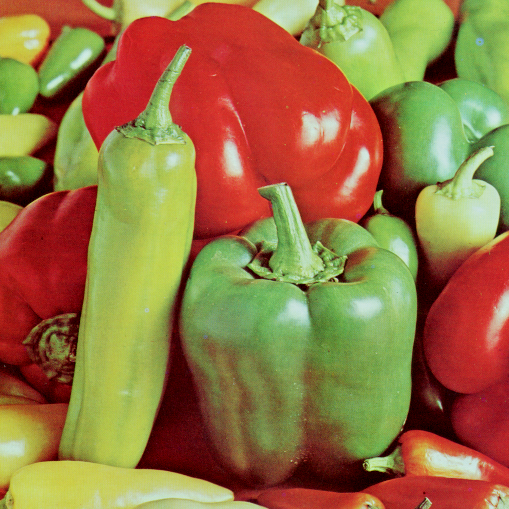
\includegraphics[width=1\textwidth]{peppers/peppers-0.png}
    \caption*{Original ($n = 0$)}
  \end{minipage}
  \hfill
  \begin{minipage}[t]{0.3\textwidth}
    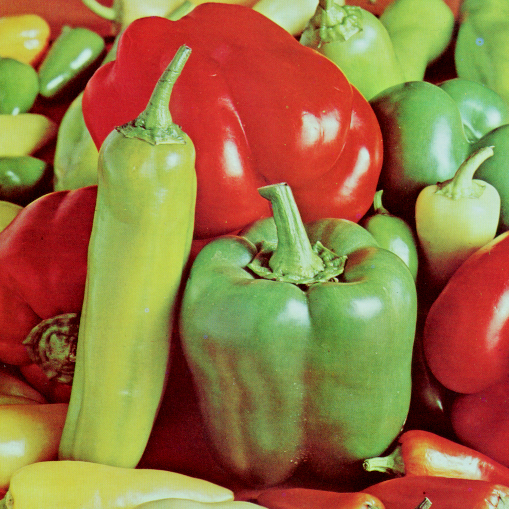
\includegraphics[width=1\textwidth]{peppers/peppers-1.png}
    \caption*{$n = 1$}
  \end{minipage}
  \hfill
  \begin{minipage}[t]{0.3\textwidth}
    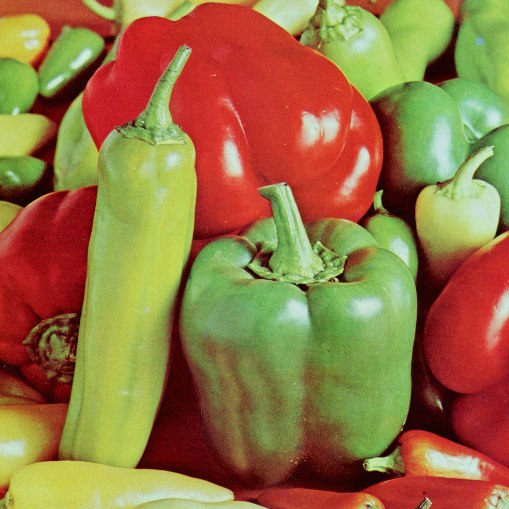
\includegraphics[width=1\textwidth]{peppers/peppers-2.png}
    \caption*{$n = 2$}
  \end{minipage}%
  \vspace{0.5cm}
  \begin{minipage}[t]{0.3\textwidth}
    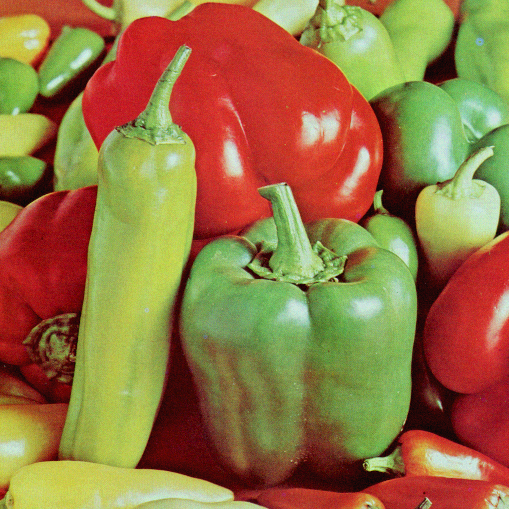
\includegraphics[width=1\textwidth]{peppers/peppers-3.png}
    \caption*{$n = 3$}
  \end{minipage}
  \hfill
  \begin{minipage}[t]{0.3\textwidth}
    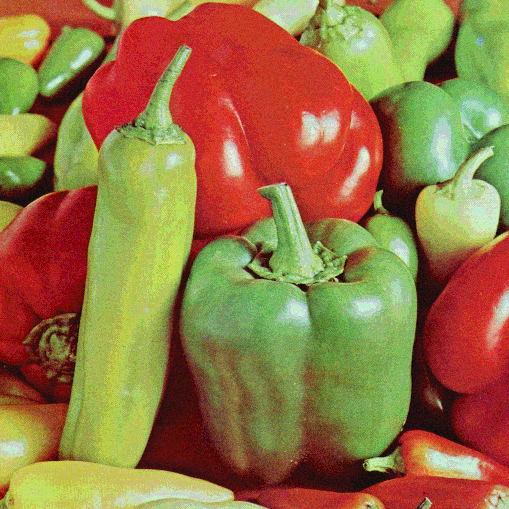
\includegraphics[width=1\textwidth]{peppers/peppers-4.png}
    \caption*{$n = 4$}
  \end{minipage}
  \hfill
  \begin{minipage}[t]{0.3\textwidth}
    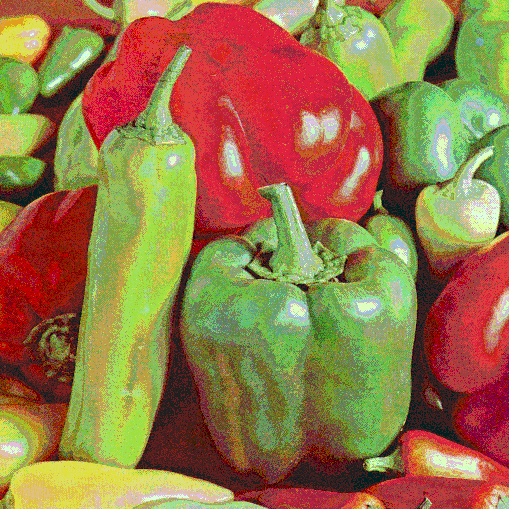
\includegraphics[width=1\textwidth]{peppers/peppers-5.png}
    \caption*{$n = 5$}
  \end{minipage}%
  \vspace{0.5cm}
  \begin{minipage}[t]{0.3\textwidth}
    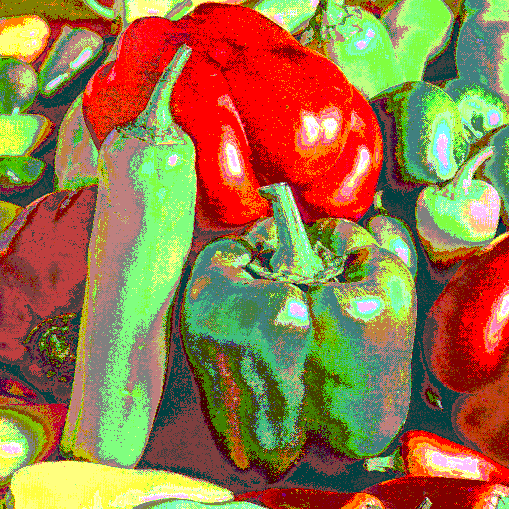
\includegraphics[width=1\textwidth]{peppers/peppers-6.png}
    \caption*{$n = 6$}
  \end{minipage}
  \hfill
  \begin{minipage}[t]{0.3\textwidth}
    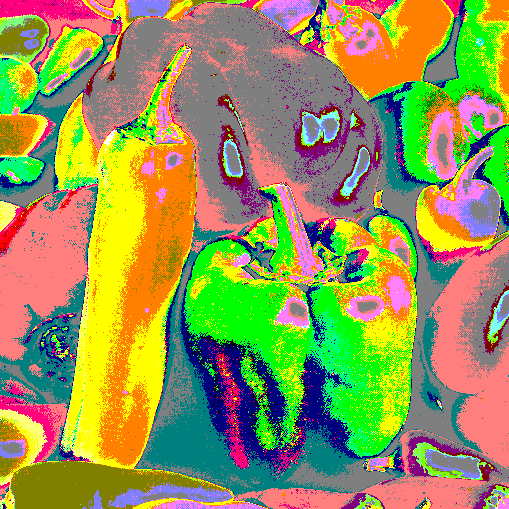
\includegraphics[width=1\textwidth]{peppers/peppers-7.png}
    \caption*{$n = 7$}
  \end{minipage}
  \hfill
  \begin{minipage}[t]{0.3\textwidth}
    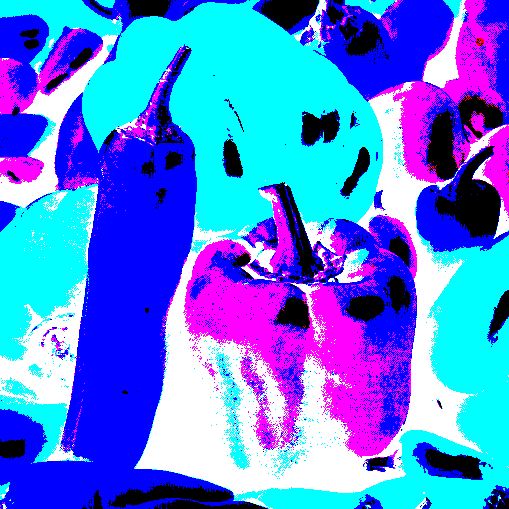
\includegraphics[width=1\textwidth]{peppers/peppers-8.png}
    \caption*{$n = 8$}
  \end{minipage}
  \caption{Farbbild Paprika verändert durch maximalen Fehler für $n \in [0,8]$.}
  \label{fig:peppers}
\end{figure}
\noindent
Zusätzlich wird in diesem Beispiel der schlimmste Fall betrachtet.
Das Verstecken einer echten Nachricht wird fast immer
ein besseres Ergebnis liefern, da Nachrichtenbit
zufällig mit den des Bilds überstimmen oder vorherige Fehler
durch weitere Teile der Nachricht wieder ausgeglichen werden.

\section{Beschreibung eines Algorithmus}
Im vorherigen Abschnitt wurden die Möglichkeiten von \acs{lsb}-Verfahren untersucht,
es kann jetzt eine mehr formale Beschreibung gegeben werden,
wie ein solcher Algorithmus umgesetzt werden kann.
Da ein steganografisches Verfahren die Vertraulichkeit einer Nachricht
nur indirekt sichert, ist es sinnvoll, diese vor dem Verwenden mit einem
kryptografischen Algorithmus zu verschlüsseln.

\begin{definition}[\acs{lsb}-Verfahren]
  Es sei $p_{xy} = (r,g,b)$ ein Pixel und $\mathbf{B} = p^{m \times n}$ ein Bild
  mit $y \in [1, m]$ und $x \in [1, n]$. Es sei $P$ die Menge aller Pixel von $\mathbf{B}$
  und $v$ eine Funktion mit $v: P \setminus \{p_{1,1},p_{m,n}\} \leftarrow v(\mathbf{B})$.
  \autoref{alg:lsb-enkodierung} und \ref{alg:lsb-dekodierung} zeigen ein Verfahren für das
  Schreiben und Lesen einer Nachricht in $\mathbf{B}$.

  \begin{singlespace}
    \begin{algorithm}
      \DontPrintSemicolon
      \KwIn{$\mathbf{B}$ und Nachricht $x$}
      \KwOut{$\mathbf{B}$ mit versteckter Nachricht $y$}
      \Begin(){
        $y \leftarrow e_k(x)$\;
        $n \leftarrow 1$\;
        schreibe Nachrichtenlänge von $y$ nach $p_{1,1}$ und $p_{m,n}$\;
        \While(){true}{
          \lIf(){$n = 9$}{$y$ ist zu lang}
          \For{$p \in v(\mathbf{B})$}{
            \For(\tcp*[f]{Farbwerte r,g,b}){$c \in p$}{
              $b \leftarrow$ lese nächstes Bit von $y$\;
              schreibe $b$ nach Position $n$ von $c$\;
              \lIf(){$y$ bearbeitet}{\Return{}}
            }
          }
          $n \leftarrow n + 1$\;
        }
      }
      \caption{\acs{lsb}-Verfahren Schreiben}
      \label{alg:lsb-enkodierung}
    \end{algorithm}
  \end{singlespace}

  \begin{singlespace}
    \begin{algorithm}[H]
      \DontPrintSemicolon
      \KwIn{$\mathbf{B}$ mit versteckter Nachricht $y$}
      \KwOut{Nachricht $x$}
      \Begin(){
        $n \leftarrow 1$\;
        $y \leftarrow \emptyset$\;
        $l \leftarrow$ lese Nachrichtenlänge bei $p_{1,1}$ und $p_{m,n}$\;
        \While(){$l \neq 0$}{
          \For(){$p \in v(\mathbf{B})$}{
            \For(\tcp*[f]{Farbwerte r,g,b}){$c \in p$}{
              $b \leftarrow$ lese Bit bei Position $n$ von $c$\;
              $y \leftarrow y \cup \{b\}$\;
              \lIf(){$l = 0$} {
                \Return{$d_k(y)$}
              }
              \lElse(){$l \leftarrow l - 1$}
            }
          }
          $n \leftarrow n + 1$\;
        }
      }
      \caption{\acs{lsb}-Verfahren Lesen}
      \label{alg:lsb-dekodierung}
    \end{algorithm}
  \end{singlespace}
\end{definition}
\noindent
Damit eine Nachricht im Bild möglichst wenig auffällt, macht es Sinn, Pixel
so auszuwählen, dass diese gleichmäßig verteilt sind. Die Verteilfunktion $v$ hat genau diese
Aufgabe. Das Bild $\mathbf{B}$ wird als Folge der natürlichen Zahlen
$a_i = 0,1,\ldots,mn - 1$ betrachtet.
Durch ein \acs{prng} wird jetzt
eine pseudozufällige Permutation von $a$ bestimmt. Der Algorithmus ist bekannt
als das Fisher-Yates-Verfahren:

\begin{singlespace}
  \begin{algorithm}[h]
    \DontPrintSemicolon
    \KwIn{Ein Array $A$ mit allen Elementen aus $a_i$ und ein \textit{seed} $s$}
    \KwOut{Permutation $A'$}
    \Begin(){
      \For(){$i \leftarrow mn - 1$ \KwTo $0$}{
        $j \leftarrow$ erzeuge pseudozufällige Zahl mit $s$ und $j \in [0,i]$\;
        tausche $A[i]$ und $A[j]$\;
      }
      \Return{$A$}\;
    }
    \caption{Fisher-Yates-Verfahren}
    \label{alg:fisher-yates-verfahren}
  \end{algorithm}
\end{singlespace}


\noindent
Der Determinismus des \acs{prng} ist wichtig, da die gleiche Permutation
für das Lesen der Nachricht ein zweites Mal erzeugt werden muss.
Durch das Lösen von $a = n \cdot y + x$ für alle $a \in A'$ mit $0 \leq x < n$
kann die Permutation in null indizierte Koordinaten $(x,y)$ des Bilds umgewandelt werden.
\begin{example}
  Ein wird ein $2 \times 3$ großes Bild betrachtet und es gilt $A' = (2,5,3,1,0,4)$.
  \begin{align*}
    2 & = 3 \cdot 0 + 2 \Rightarrow (2,0)          \\
    5 & = 3 \cdot 1 + 2 \Rightarrow (2,1)          \\
    3 & = 3 \cdot 1 + 0 \Rightarrow (0,1)          \\
    1 & = 3 \cdot 0 + 1 \Rightarrow (1,0)          \\
    0 & = 3 \cdot 0 + 0 \Rightarrow (0,0)          \\
    4 & = 3 \cdot 1 + 1 \Rightarrow (1,1) \qedhere
  \end{align*}
\end{example}

\noindent
\autoref{fig:punkt-verteilung} zeigt die Koordinatenverteilung für Nachrichten unterschiedlicher
Längen auf einem $500 \times 500$ Pixel Farbbild mit schwarzen Hintergrund. Die durch den Algorithmus
errechneten Koordinaten sind weiß eingefärbt.

\begin{figure}
  \centering
  \begin{tikzpicture}
    [spy scope= {circle, magnification=3, size=2cm},
      every spy in node/.style={draw, Red, thin},
      every node/.style={inner sep=0},
      label distance=-0.5cm]

    \node (1200b) {
      \begin{minipage}{0.45\textwidth}
        
\includegraphics[width=1\textwidth]{black/black-1200.png}
        \caption*{1200 Byte}
      \end{minipage}
    };
    \node [right= of 1200b] (3600b) {
      \begin{minipage}{0.45\textwidth}
        
\includegraphics[width=1\textwidth]{black/black-3600.png}
        \caption*{3600 Byte}
      \end{minipage}
    };
    \node [below=0.5cm of 1200b] (10800b) {
      \begin{minipage}{0.45\textwidth}
        
\includegraphics[width=1\textwidth]{black/black-10800.png}
        \caption*{10800 Byte}
      \end{minipage}
    };
    \node [below=0.5cm of 3600b] (32400b) {
      \begin{minipage}{0.45\textwidth}
        
\includegraphics[width=1\textwidth]{black/black-32400.png}
        \caption*{32400 Byte}
      \end{minipage}
    };

    \matrix [column sep=2.5cm] at ($(1200b.north)!0.5!(3600b.north) + (0,2.5cm)$) {
      \coordinate (a); & \coordinate (b); & \coordinate (c); & \coordinate (d); \\
    };

    \spy on ($(1200b.north) + (2cm,-4.1cm)$) in node;
    \spy on ($(1200b.north) + (-2cm,-2cm)$) in node;

    \spy on ($(3600b.north) + (2cm,-1.3cm)$) in node;
    \spy on ($(3600b.north) + (-2cm,-3cm)$) in node;

    \spy on ($(10800b.north) + (2cm,-5.5cm)$) in node;
    \spy on ($(10800b.north) + (-2cm,-2.25cm)$) in node;

    \spy on ($(32400b.north) + (2cm,-2.8cm)$) in node;
    \spy on ($(32400b.north) + (-2cm,-5cm)$) in node;

  \end{tikzpicture}
  \caption{Koordinatenverteilung auf einem $500 \times 500$ Pixel Farbbild mit
    schwarzen Hintergrund für Nachrichtenlängen von 1200, 3600, 10800 und 32400 Byte.}
  \label{fig:punkt-verteilung}
\end{figure}


\newpage
\section{Die Architektur der Anwendung}
Es soll jetzt auf die zu Beginn des Kapitels beschrieben Anwendung
eingegangen werden, welche im Rahmen dieser Studienarbeit entwickelt wurde.
Die Anwendung muss verschiedene Benutzer verwalten können und
einen sicheren Nachrichtenaustausch über in Bildern
versteckten Informationen gewährleisten.
Die wichtigsten Sicherheitsaspekte eines
solchen Systems sind die Folgenden:
\begin{enumerate}
  \item \textbf{Vertraulichkeit} einer Nachricht (Geheimhaltung, Verschlüsselung).
  \item \textbf{Integrität} einer Nachricht (Hashfunktion, \acp{mac}).
  \item \textbf{Authentizität} des Empfängers. Es darf nicht passieren, der falschen Person
        unwissentlich eine geheime Nachricht zu senden. Im Rahmen dieser Betrachtung sollte
        es reichen, nicht zwei Personen mit demselben Benutzernamen zuzulassen.
  \item \textbf{Authentifizierung} und \textbf{Autorisierung}. Um eine Nachricht
        (z.\,B. für das Schreiben im Bild) benutzergebunden zu verschlüsseln,
        müssen Anfragen immer klar mit einem Benutzer in Verbindung gebracht werden.
\end{enumerate}

\noindent
Die verschiedenen Teile der Anwendung können unterteilt werden in die
drei Bereiche: Präsentation, Schnittstelle und Persistenz.
Benutzer müssen angemeldet sein, um auf geschützte Bereiche der Schnittstelle zuzugreifen.
Es wurde eine Token basierte Autorisierung gewählt, welche mithilfe von \acp{jwt}
implementiert ist. \ac{jwt} ist ein Internet Standard (RFC 7519, \cite{SITE:jwt}) und ein
weit verbreitetes Verfahren für die Autorisierung im Web und \textit{Single Sign-On} Anwendungen.
\autoref{fig:jwt-auth} zeigt einen typischen Anfrageablauf zwischen Anwender und einer Anwendung
mit \acs{jwt} Autorisierung.
\newpage

\begin{figure}[h]
  \centering
  \begin{tikzpicture}
    [node distance=0.5cm,
      op/.style={draw=blue, inner xsep=0.5em, fill=blue!10 }]

    \coordinate (user) at (0,-1);
    \coordinate (api) at (6,-1);
    \coordinate (auth) at (12,-1);

    \draw[dashed] (user) -- (0,-12);
    \draw[dashed] (api) -- (6,-12);
    \draw[dashed] (auth) -- (12,-12);

    \node[above= of user]{\textbf{Benutzer}};

    \node[above= of api, align=center]{\textbf{API} \\ \textbf{(Ressourcen Server)}};

    \node[below=3cm of api, op, inner ysep=4em] (endpoint-1) {};
    \draw[<-] ([yshift=-1.5em]$(endpoint-1.north west)$) --
    node[above, font=\scriptsize] {Anfrage + Token} ++($(-6,0) + (0.5em,0)$);
    \draw[->] ([yshift=-2.5em]$(endpoint-1.north west)$) --
    node[below, font=\scriptsize] {2xx} ++($(-6,0) + (0.5em,0)$);
    \draw[<-] ([yshift=2.5em]$(endpoint-1.south west)$) --
    node[above, font=\scriptsize] {Anfrage + Abgelaufener Token} ++($(-6,0) + (0.5em,0)$);
    \draw[->] ([yshift=1.5em]$(endpoint-1.south west)$) --
    node[below, font=\scriptsize] {401} ++($(-6,0) + (0.5em,0)$);

    \begin{scope}
      \clip (5,-12.1) rectangle (7,-10);
      \node[op, inner ysep=3em] (endpoint-2) at (6,-12) {};
    \end{scope}
    \draw[<-] ([yshift=-1.5em]$(endpoint-2.north west)$) --
    node[above, font=\scriptsize] {Anfrage + Token} ++($(-6,0) + (0.5em,0)$);

    \node[above= of auth, align=center]{\textbf{Autorisierungs-} \\ \textbf{server}};

    \node[below= of auth, op, inner ysep=2em] (login) {};
    \draw[<-] ([yshift=0.5em]$(login.west)$) --
    node[above, near end, font=\scriptsize] {Login/Register} ++($(-12,0) + (0.5em,0)$);
    \draw[->] ([yshift=-0.5em]$(login.west)$) --
    node[below, near start, font=\scriptsize] {(Token, Erneuerungstoken)} ++($(-12,0) + (0.5em,0)$);

    \node[below=7cm of auth, op, inner ysep=2em] (refresh) {};
    \draw[<-] ([yshift=0.5em]$(refresh.west)$) --
    node[above, near end, font=\scriptsize] {(Abgelaufener Token, Erneuerungstoken)} ++($(-12,0) + (0.5em,0)$);
    \draw[->] ([yshift=-0.5em]$(refresh.west)$) --
    node[below, near start, font=\scriptsize] {(Token, Erneuerungstoken)} ++($(-12,0) + (0.5em,0)$);

    \node[cylinder, draw, rotate=90, minimum width=1cm, minimum height=1cm,
      label={[font=\scriptsize]180:Benutzer Datenbank}] at (9,-4.5) {}
    edge[<->, shorten >= 0.5em, shorten <= 0.5em] (login.south west);
  \end{tikzpicture}
  \caption{Sequenzdiagramm \acs{jwt} Autorisierung}
  \label{fig:jwt-auth}
\end{figure}

\noindent
Ein Benutzer erhält nach dem Anmelden eine Kombination aus Zugriffstoken
(engl. \textit{access token}) und Erneuerungstoken (engl. \textit{refresh token}),
welche clientseitig gespeichert werden.
Wird versucht, auf einen geschützten Bereich der API zuzugreifen, muss die Anfrage
einen gültigen Token enthalten, welcher als Teil des HTTP-Header im
Autorisierungsfeld versandt wird.
Ist im Header der Anfrage kein oder ein
abgelaufener Token vorhanden, wird diese mit einem HTTP-Statuscode 401 \enquote{Unautorisiert}
abgelehnt. Ist ein Token abgelaufen, kann dieser beim Autorisierungsserver
zusammen mit dem Erneuerungstoken aktualisiert werden.

\section{Sicherheitsanalyse}
Es soll nun weiter auf die beschriebene Architektur der Anwendung eingegangen werden,
mit dem Ziel, Sicherheitsbedenken aufzudecken und Lösungen zu diskutieren.
Anschließend wird die steganografische Qualität des Algorithmus
untersucht und einige Beispiele gezeigt.

\subsection{Risiken der Token basierten Autorisierung}
Besondere Vorsicht muss geboten werden, wenn es um die Handhabung
der Zugriffstoken geht.
Fällt ein Token in die Hände eines Angreifers, kann dieser
im Namen des Tokeninhabers beliebig Anfragen durchführen, d.\,h. sowohl geheime Nachrichten
lesen als auch Nachrichten schreiben.
Zugriffstoken werden clientseitig gespeichert. Über eine
Clientumgebung wie beispielsweise dem Webbrowser, besteht in den meisten
Fällen keine 100-prozentige Kontrolle, weshalb die volle Sicherheit hier leider nicht
garantiert sein kann. Dennoch sollten Sicherheitsmaßnahmen getroffen werden, um
das Risiko eines Missbrauchs zu verringern.
Um den Zeitraum von Angriffsmöglichkeiten kurz zu halten, sollte
ein Token nur so lange gültig sein wie nötig
(z.\,B. nicht länger als fünf Minuten).
Es existieren zwei wesentliche Angriffstypen, welche das Prinzip der Token Autorisierung
versuchen auszunutzen. Die folgende Überlegung ist beschränkt auf die Domäne
der Webanwendungen:

\paragraph{Cross-Site-Scripting (XSS)}
Schafft es ein Angreifer auf einer Webseite an der richtigen Stelle
ein Stück JavaScript auszuführen,
kann er mit den richtigen Befehlen den Zugriffstoken ganz einfach auslesen.
Webseiten sollten daher an Stellen wie Benutzereingaben vorsichtig sein und diese
beispielsweise nie direkt als Teil des HTML anzeigen lassen.

\paragraph{Cross-Site-Request-Forgery (CSRF)}
CSRF-Angriffe zielen darauf ab, HTTP-An\-fragen im
Namen anderer Benutzer durchzuführen. Sie machen dabei Gebrauch von
aktiven Sitzungen oder im Falle der Token Autorisierung von Zugriffstoken,
welche pro Anfrage automatisch (z.\,B. per Cookie) versandt werden.
Zugriffstoken sollten somit nie direkt als Cookie gespeichert werden. Besser
ist es, Sitzungen indirekt über Erneuerungstoken aufrechtzuerhalten oder
in extremen Fällen gar keine Sitzungsinformationen zu speichern.

\noindent
Die Zugriffstoken der hier beschriebenen Anwendung haben eine Gültigkeitsdauer
von 30 Sekunden und es werden keine Sitzungsinformationen gespeichert.

\subsection{Kryptografische Qualität}
Nachrichten werden verschlüsselt, bevor sie in einem Bild versteckt werden.
Verschlüssel\-ung geschieht durch die \textit{ASP.NET Core Data Protection API}
, welche als sicher angenommen wird. \footnote{https://docs.microsoft.com/en-us/aspnet/core/\\
  security/data-protection/introduction?view=aspnetcore-5.0}
Als Garantie, dass nur der geplante Empfänger eine Nachricht lesen
kann, ist ein eindeutiger \textit{purposes parameter} nötig, welcher
der Verschlüsselungsfunktion übergeben wird.
Der Parameter setzt sich zusammen aus (Datenbank ID $\parallel$ - $\parallel$ Name)
und ist somit garantiert eindeutig, das Symbol $\parallel$
beschreibt hierbei die Konkatenation zweier Zeichenketten.
\autoref{alg:data-protect} und \ref{alg:data-unprotect}
zeigen das Prinzip der Verschlüsselung. Die \textit{Data Protection API} stellt
eine Methode \texttt{CreateProtector} zur Verfügung:

\begin{singlespace}
  \begin{algorithm}[h]
    \DontPrintSemicolon
    \KwIn{message $x$ and information of the receiver $(id,username)$}
    \KwOut{protected message $y$}
    \Begin(){
      $(e_k, d_k) \leftarrow$ \texttt{CreateProtector}($id \parallel \text{-} \parallel username$)\;
      \Return{$e_k(x)$}
    }
    \caption{\textit{Data Protection Encryption}}
    \label{alg:data-protect}
  \end{algorithm}
\end{singlespace}

\noindent
Es ist nun zu sehen, warum es wichtig ist, Anfragen mit einem Benutzer in Verbindung zu bringen:

\begin{singlespace}
  \begin{algorithm}[h]
    \DontPrintSemicolon
    \KwIn{protected message $y$}
    \KwOut{message $x$}
    \Begin(){
      $(id, username) \leftarrow$ get user information of request\;
      $(e_k, d_k) \leftarrow$ \texttt{CreateProtector}($id \parallel \text{-} \parallel username$)\;
      \Return{$d_k(y)$}
    }
    \caption{\textit{Data Protection Decryption}}
    \label{alg:data-unprotect}
  \end{algorithm}
\end{singlespace}

\noindent
Das Funktionspaar $(e_k, d_k)$ der \texttt{CreateProtector} Methode verwendet \acp{mac},
um die unbemerkte Nachrichtenmanipulation zu verhindern. Wäre die Nachricht während der Übertragung
verändert worden, würde es während der Entschlüsselung auffallen.

\newcommand{\bmax}{\ensuremath{\mathbf{B}_{max}}}

\subsection{Steganografische Qualität}
Um die Qualität des steganografischen Algorithmus zu beurteilen,
lohnt es sich vor allem einige
Beispiele anzusehen.
Nach der Überlegung in \autoref{sec:bild-these} können wir abschätzen,
wie lang eine Nachricht sein sollte, um mit
den Beispielbildern sinnvolle Beobachtungen machen zu können.
Die nachfolgende Tabelle
zeigt die nötige Länge einer Nachricht, um auf allen $n$ \acs{lsb}
der Farbkanäle Änderungen auszulösen.
Die Nachrichtenlänge $l$ ist als prozentualer Anteil
der maximalen Bildkapazität $\bmax$ angegeben:
\begin{table}[h]
  \centering
  \caption{Die Zuordnung von $n$ zu der Nachrichtenlänge $l$ in Bezug auf $\bmax$}
  \begin{tabular}{|c|c|}
    \hline
    n & $l$        \\ \hline
    0 & \num{0}    \\ \hline
    1 & \num{12,5} \\ \hline
    2 & \num{25}   \\ \hline
    3 & \num{37,5} \\ \hline
    4 & \num{50}   \\ \hline
    5 & \num{62,5} \\ \hline
    6 & \num{75}   \\ \hline
    7 & \num{87,5} \\ \hline
    8 & \num{100}  \\ \hline
  \end{tabular}
  \label{tab:zuordnung-n-bmax}
\end{table}

\noindent
Es macht keinen Sinn, Nachrichten zu betrachten mit $l < \num{37.5}\,\%$,
da diese in den allermeisten Fällen eine gute Bildqualität aufweisen.
Zusätzlich macht es keinen Sinn, sehr lange Nachrichten zu
untersuchen, da diese immer eine schlechte Bildqualität erzeugen.
In den folgenden Beispielen wird deshalb nur der mittlere Bereich $n \in [4,6]$ beachtet.
Es werden jeweils drei Bilder miteinander verglichen mit einer
versteckten Nachrichtenlänge von 48, 60 und 72\,\% der maximalen Bildkapazität.
Die Nachrichten sind jeweils zufällig erzeugt:

\newpage

\begin{figure}[h!]
  \centering
  \begin{tikzpicture}
    [spy scope= {circle, magnification=6, size=3cm},
      every spy on node/.style={draw, blue, thick},
      every node/.style={inner sep=0},
      label distance=-1cm]

    \node (original) {
      \begin{minipage}{0.35\textwidth}
        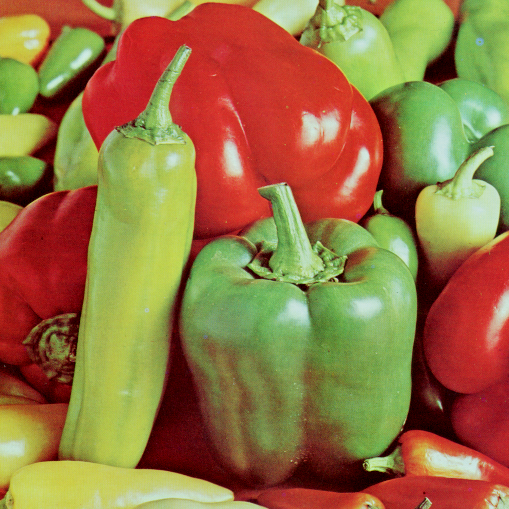
\includegraphics[width=1\textwidth]{peppers/peppers-0.png}
        \caption*{Original}
      \end{minipage}
    };
    \node [right= of original] (300kb) {
      \begin{minipage}{0.35\textwidth}
        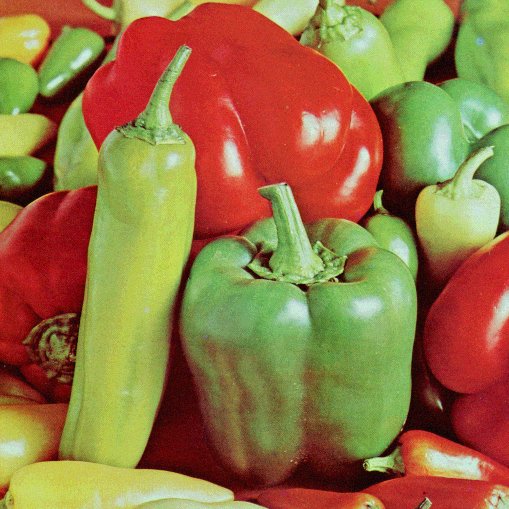
\includegraphics[width=1\textwidth]{peppers/peppers-48.png}
        \caption*{48\,\% (373\,kB)}
      \end{minipage}
    };
    \node [below=0.5cm of original] (500kb) {
      \begin{minipage}{0.35\textwidth}
        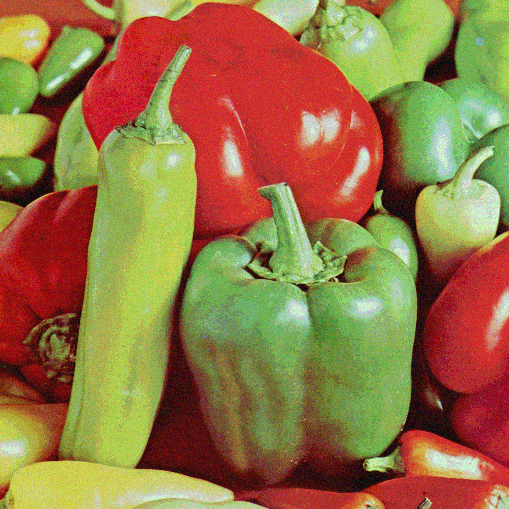
\includegraphics[width=1\textwidth]{peppers/peppers-60.png}
        \caption*{60\,\% (466\,kB)}
      \end{minipage}
    };
    \node [below=0.5cm of 300kb] (700kb) {
      \begin{minipage}{0.35\textwidth}
        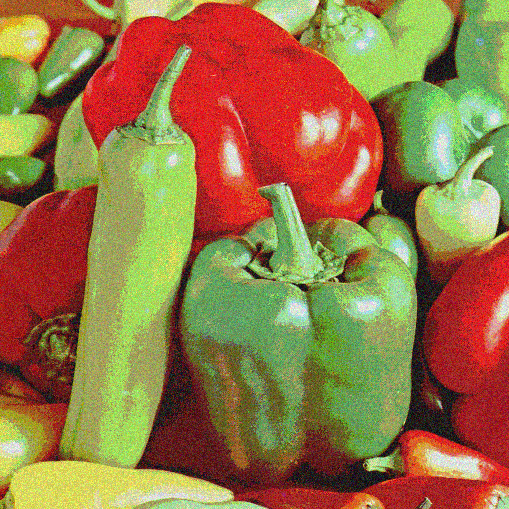
\includegraphics[width=1\textwidth]{peppers/peppers-72.png}
        \caption*{72\,\% (560\,kB)}
      \end{minipage}
    };

    \matrix [column sep=3.5cm] at ($(original.north)!0.5!(300kb.north) + (0,3.5cm)$) {
      \coordinate (a); & \coordinate (b); & \coordinate (c); & \coordinate (d); \\
    };

    \coordinate (spy-on) at (-0.95cm,-0.8cm);

    \spy on ($(original.north) + (spy-on)$) in node[label=below:Original] at (a);
    \spy on ($(300kb.north) + (spy-on)$) in node[label=below:48\,\%] at (b);
    \spy on ($(500kb.north) + (spy-on)$) in node[label=below:60\,\%] at (c);
    \spy on ($(700kb.north) + (spy-on)$) in node[label=below:72\,\%] at (d);


  \end{tikzpicture}
  \caption{Paprika mit einer Größe von 509 $\times$ 509 Pixel.
    Gute Bildqualität zwischen 373 und 466\,kB versteckter Nachricht ($\bmax \approx 777$\,kB).}
  \label{fig:example-peppers}
\end{figure}


\newpage

\begin{figure}[h!]
  \centering
  \begin{tikzpicture}
    [spy scope= {circle, magnification=8, size=3cm},
      every spy on node/.style={draw, Red, ultra thick},
      every node/.style={inner sep=0},
      label distance=-1cm]

    \node (original) {
      \begin{minipage}{0.45\textwidth}
        \includegraphics[width=1\textwidth]{turtle.png}
        \caption*{Original}
      \end{minipage}
    };
    \node [right= of original] (2mb) {
      \begin{minipage}{0.45\textwidth}
        \includegraphics[width=1\textwidth]{turtle-2000000.png}
        \caption*{2 MB Nachricht}
      \end{minipage}
    };
    \node [below=0.5cm of original] (4mb) {
      \begin{minipage}{0.45\textwidth}
        \includegraphics[width=1\textwidth]{turtle-4000000.png}
        \caption*{4 MB Nachricht}
      \end{minipage}
    };
    \node [below=0.5cm of 2mb] (6mb) {
      \begin{minipage}{0.45\textwidth}
        \includegraphics[width=1\textwidth]{turtle-6000000.png}
        \caption*{6 MB Nachricht}
      \end{minipage}
    };

    \matrix [column sep=3.5cm] at ($(original.north)!0.5!(2mb.north) + (0,3.5cm)$) {
      \coordinate (a); & \coordinate (b); & \coordinate (c); & \coordinate (d); \\
    };

    \coordinate (spy-on) at (1cm,-0.5cm);

    \spy on ($(original.north) + (spy-on)$) in node[label=below:Original] at (a);
    \spy on ($(2mb.north) + (spy-on)$) in node[label=below:2 MB] at (b);
    \spy on ($(4mb.north) + (spy-on)$) in node[label=below:4 MB] at (c);
    \spy on ($(6mb.north) + (spy-on)$) in node[label=below:6 MB] at (d);


  \end{tikzpicture}
  \caption{Schildkröte. Größe 1368 $\times$ 1824 Pixel. Maximale Kapazität $\approx 7,5$ MB.
    Gute Bildqualität bis zu 4MB versteckter Nachricht.}
  \label{fig:example-turtle}
\end{figure}


\newpage

\begin{figure}[h!]
  \centering
  \begin{tikzpicture}
    [spy scope= {circle, magnification=6, size=3cm},
      every spy on node/.style={draw, Red, thick},
      every node/.style={inner sep=0},
      label distance=-1cm]

    \node (original) {
      \begin{minipage}{0.45\textwidth}
        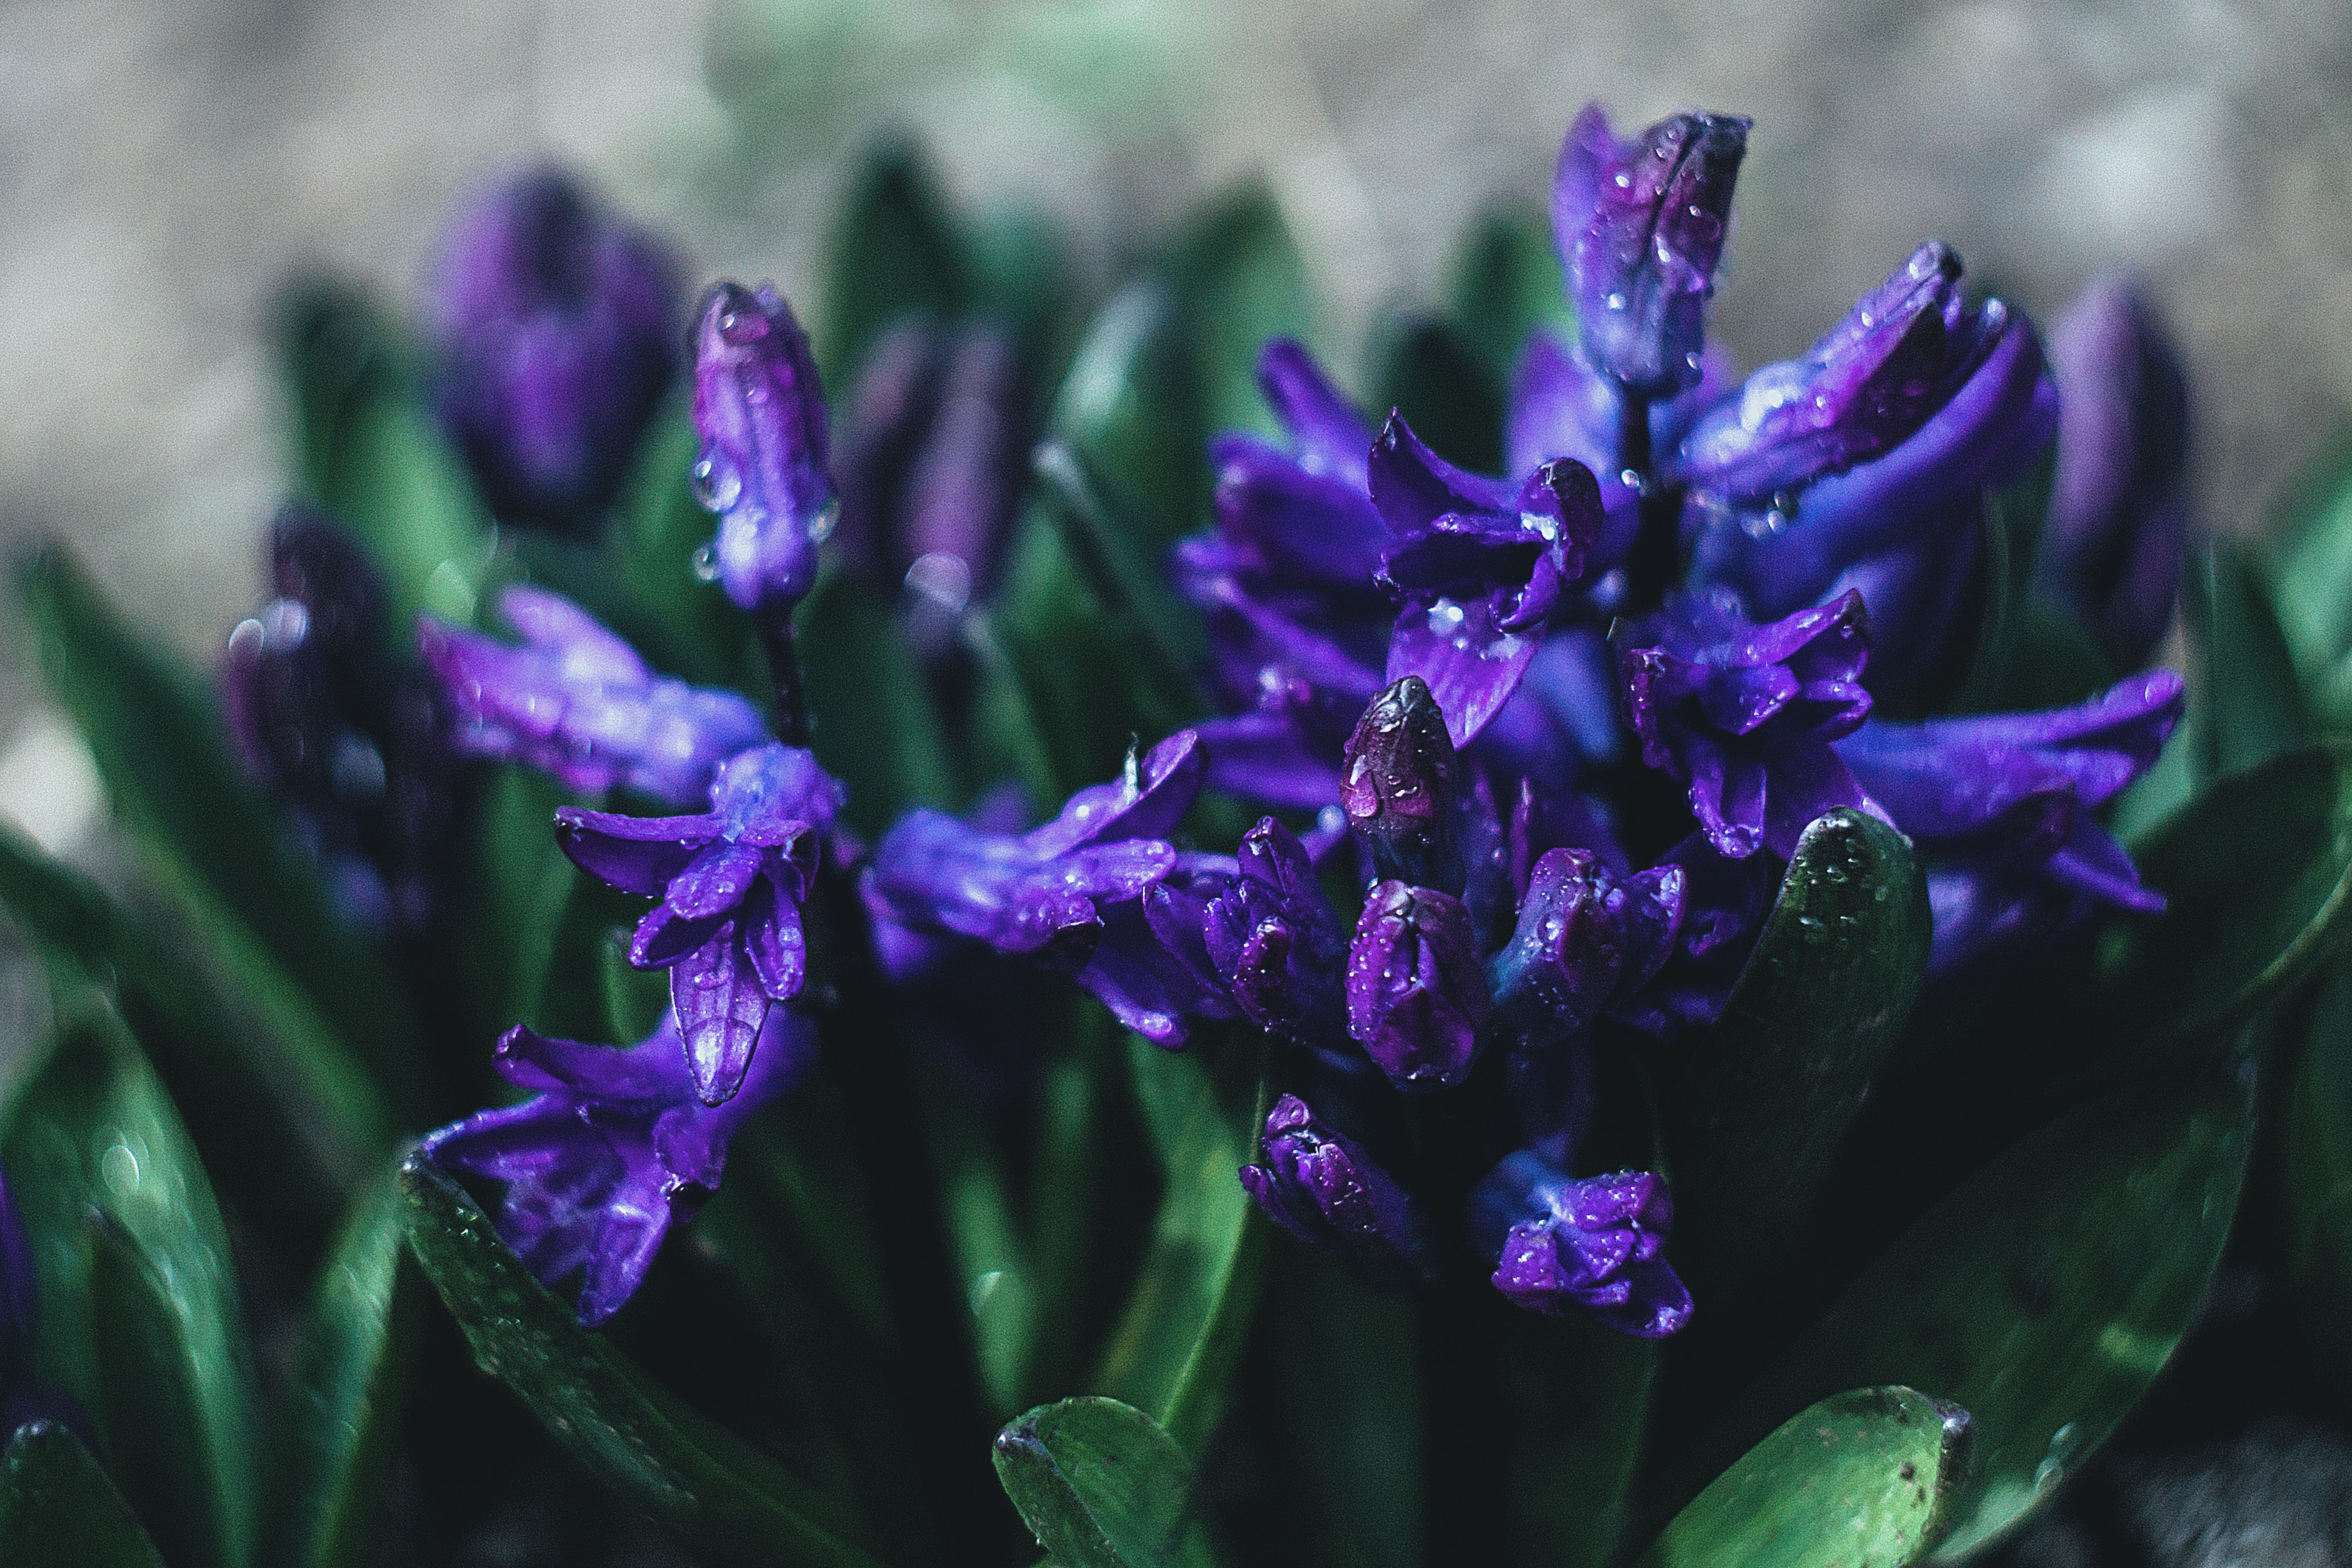
\includegraphics[width=1\textwidth]{flowers/flowers.png}
        \caption*{Original}
      \end{minipage}
    };
    \node [right= of original] (10mb) {
      \begin{minipage}{0.45\textwidth}
        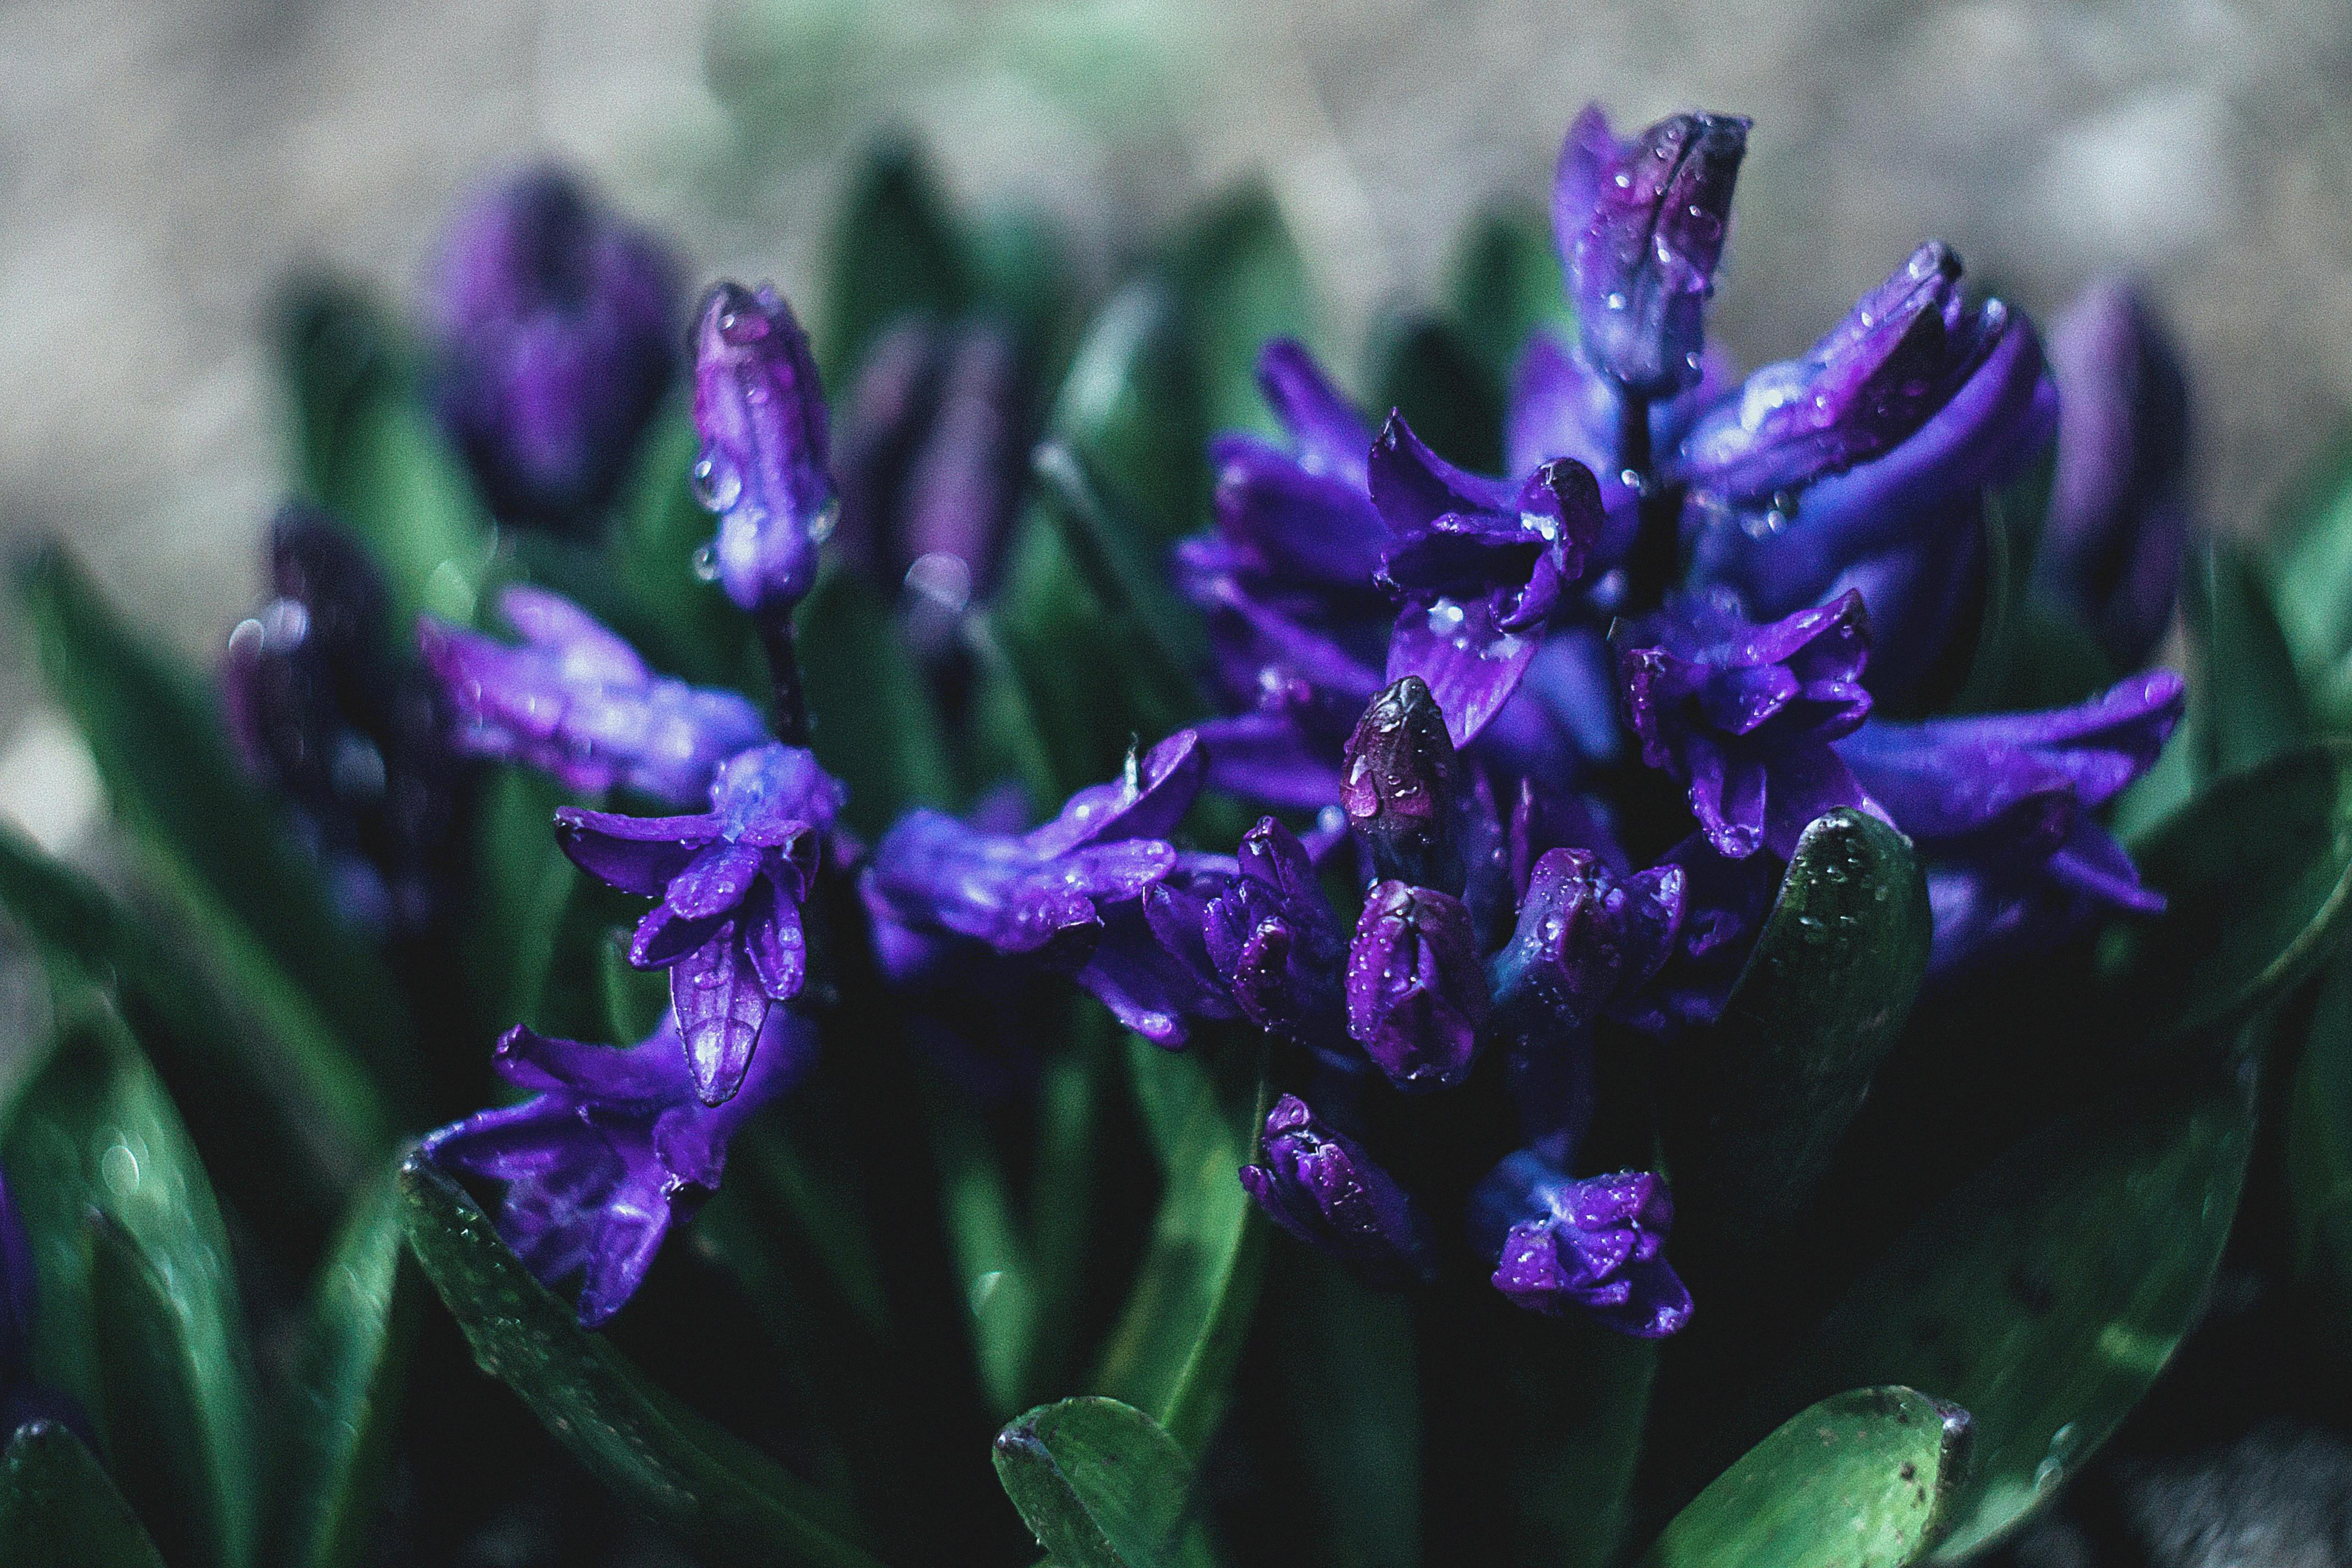
\includegraphics[width=1\textwidth]{flowers/flowers-48.png}
        \caption*{48\,\% (\num{17.5}\,MB)}
      \end{minipage}
    };
    \node [below=0.5cm of original] (20mb) {
      \begin{minipage}{0.45\textwidth}
        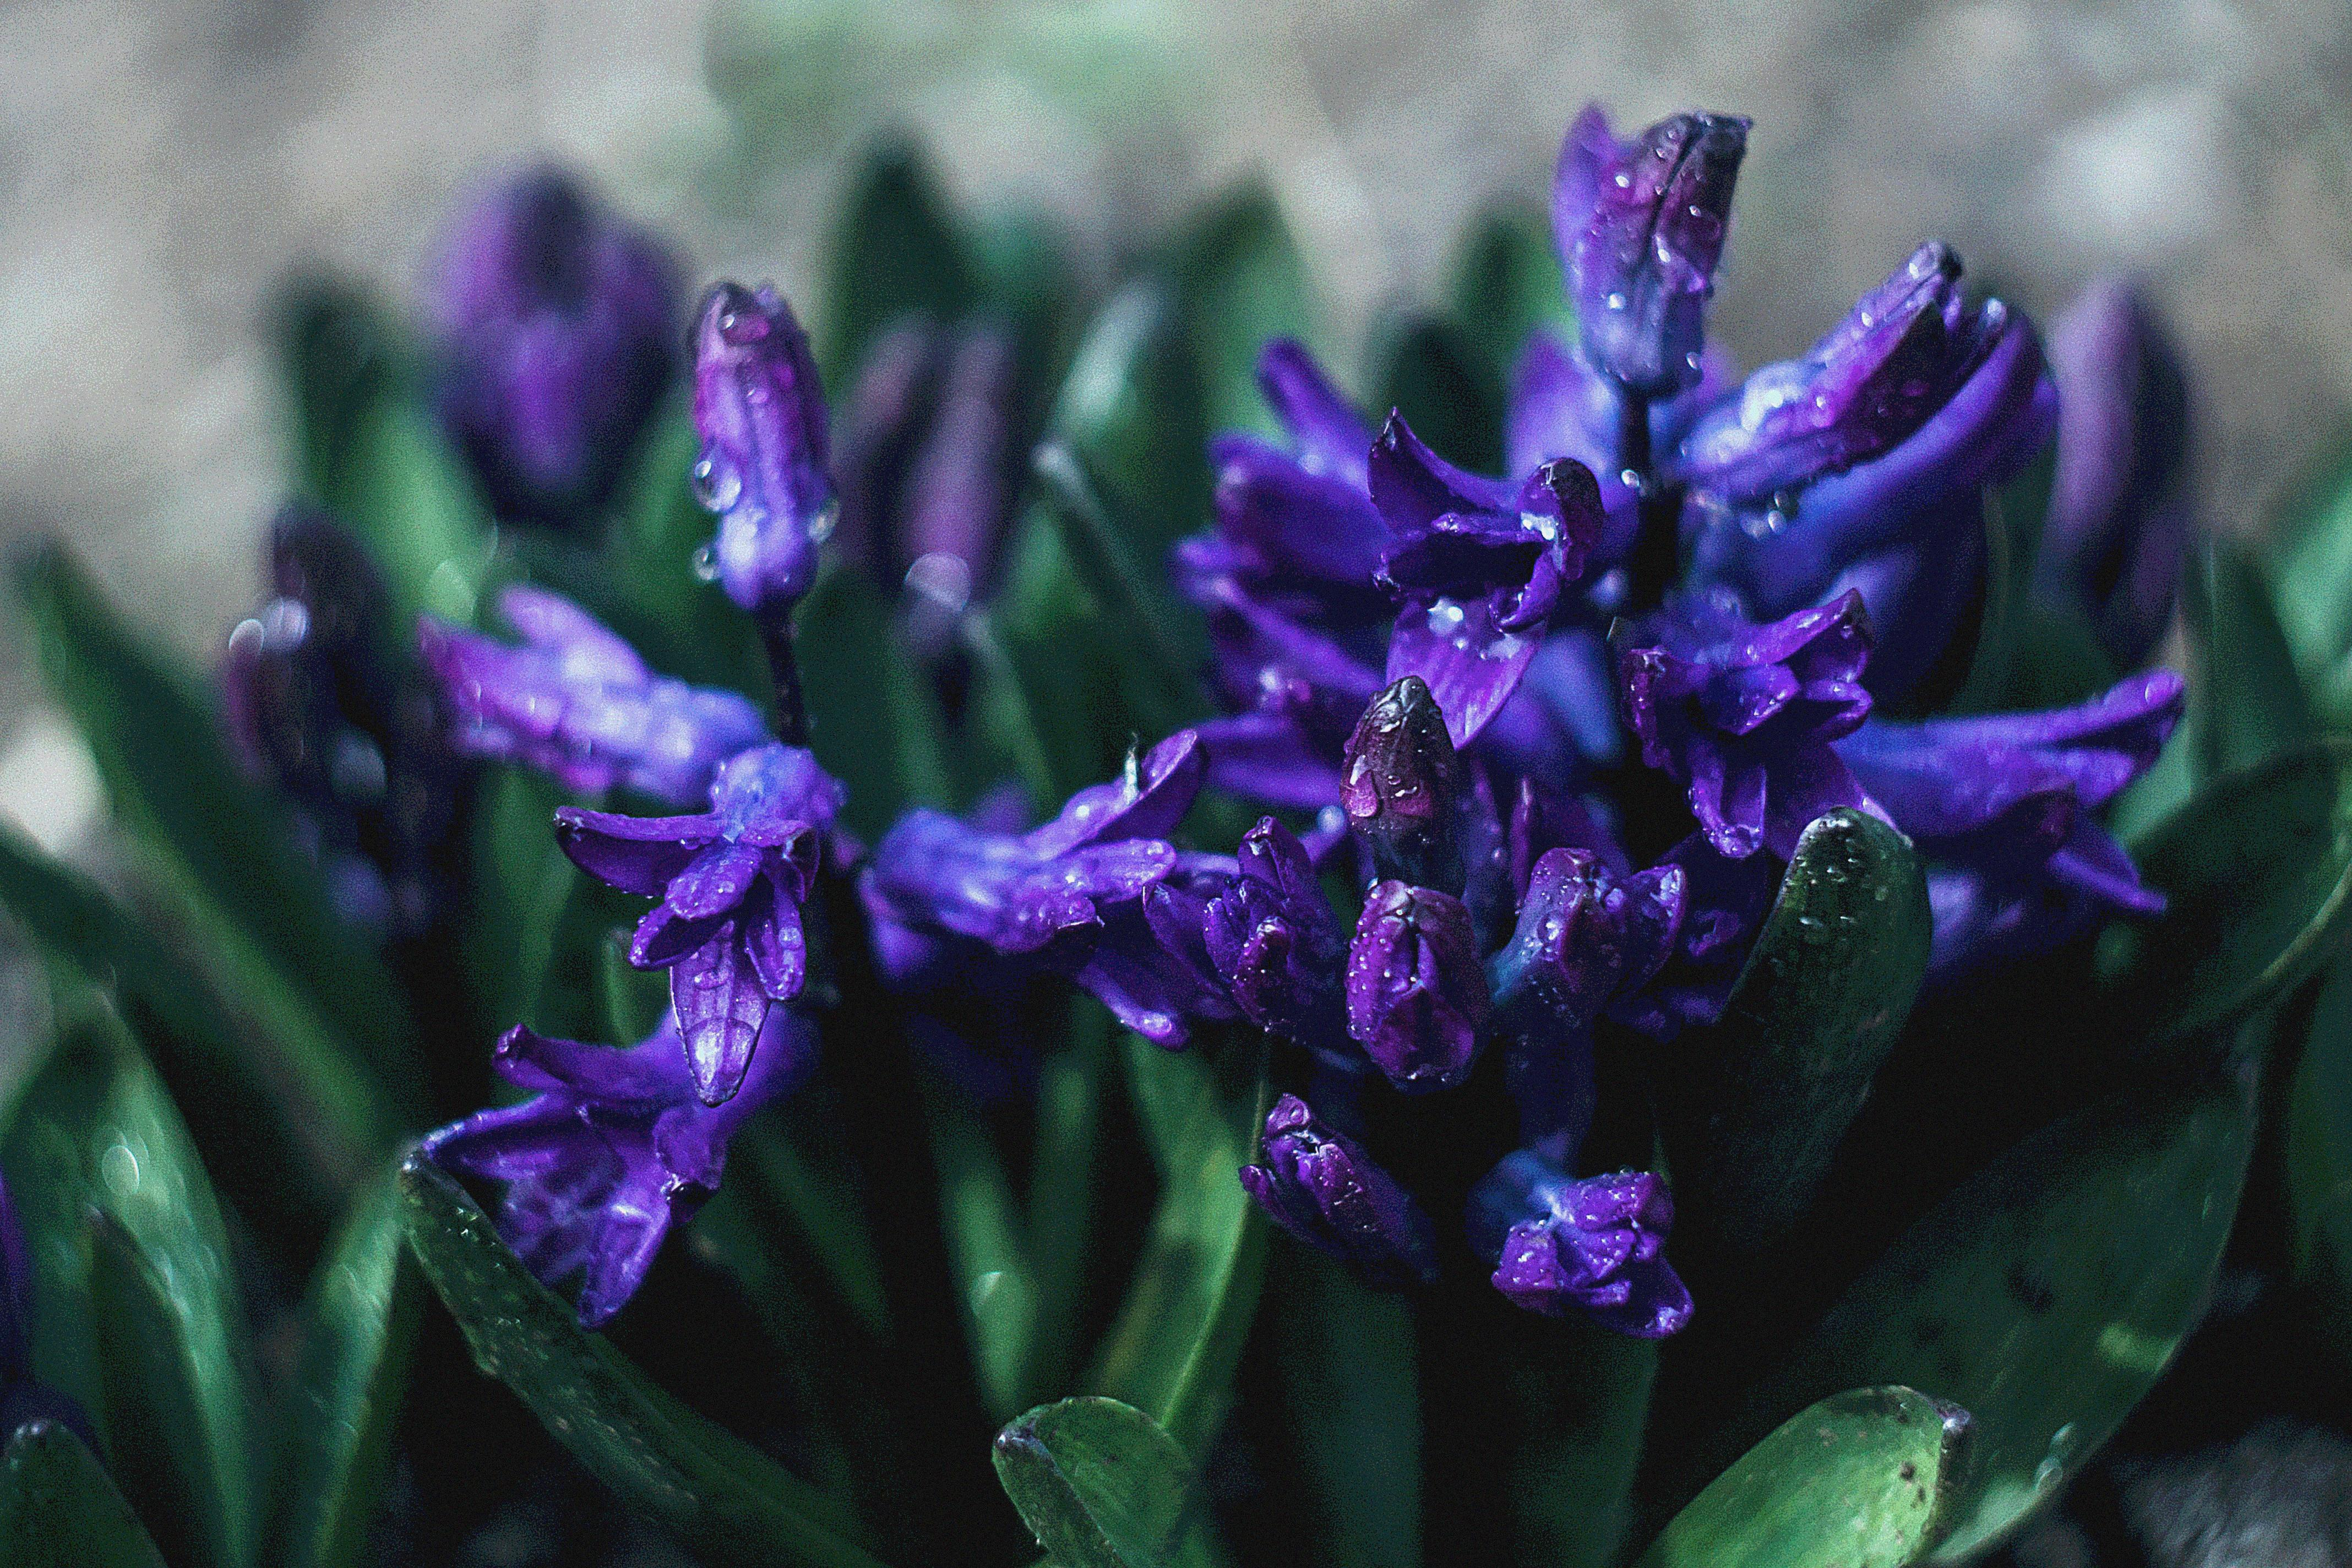
\includegraphics[width=1\textwidth]{flowers/flowers-60.png}
        \caption*{60\,\% (\num{21.9}\,MB)}
      \end{minipage}
    };
    \node [below=0.5cm of 10mb] (30mb) {
      \begin{minipage}{0.45\textwidth}
        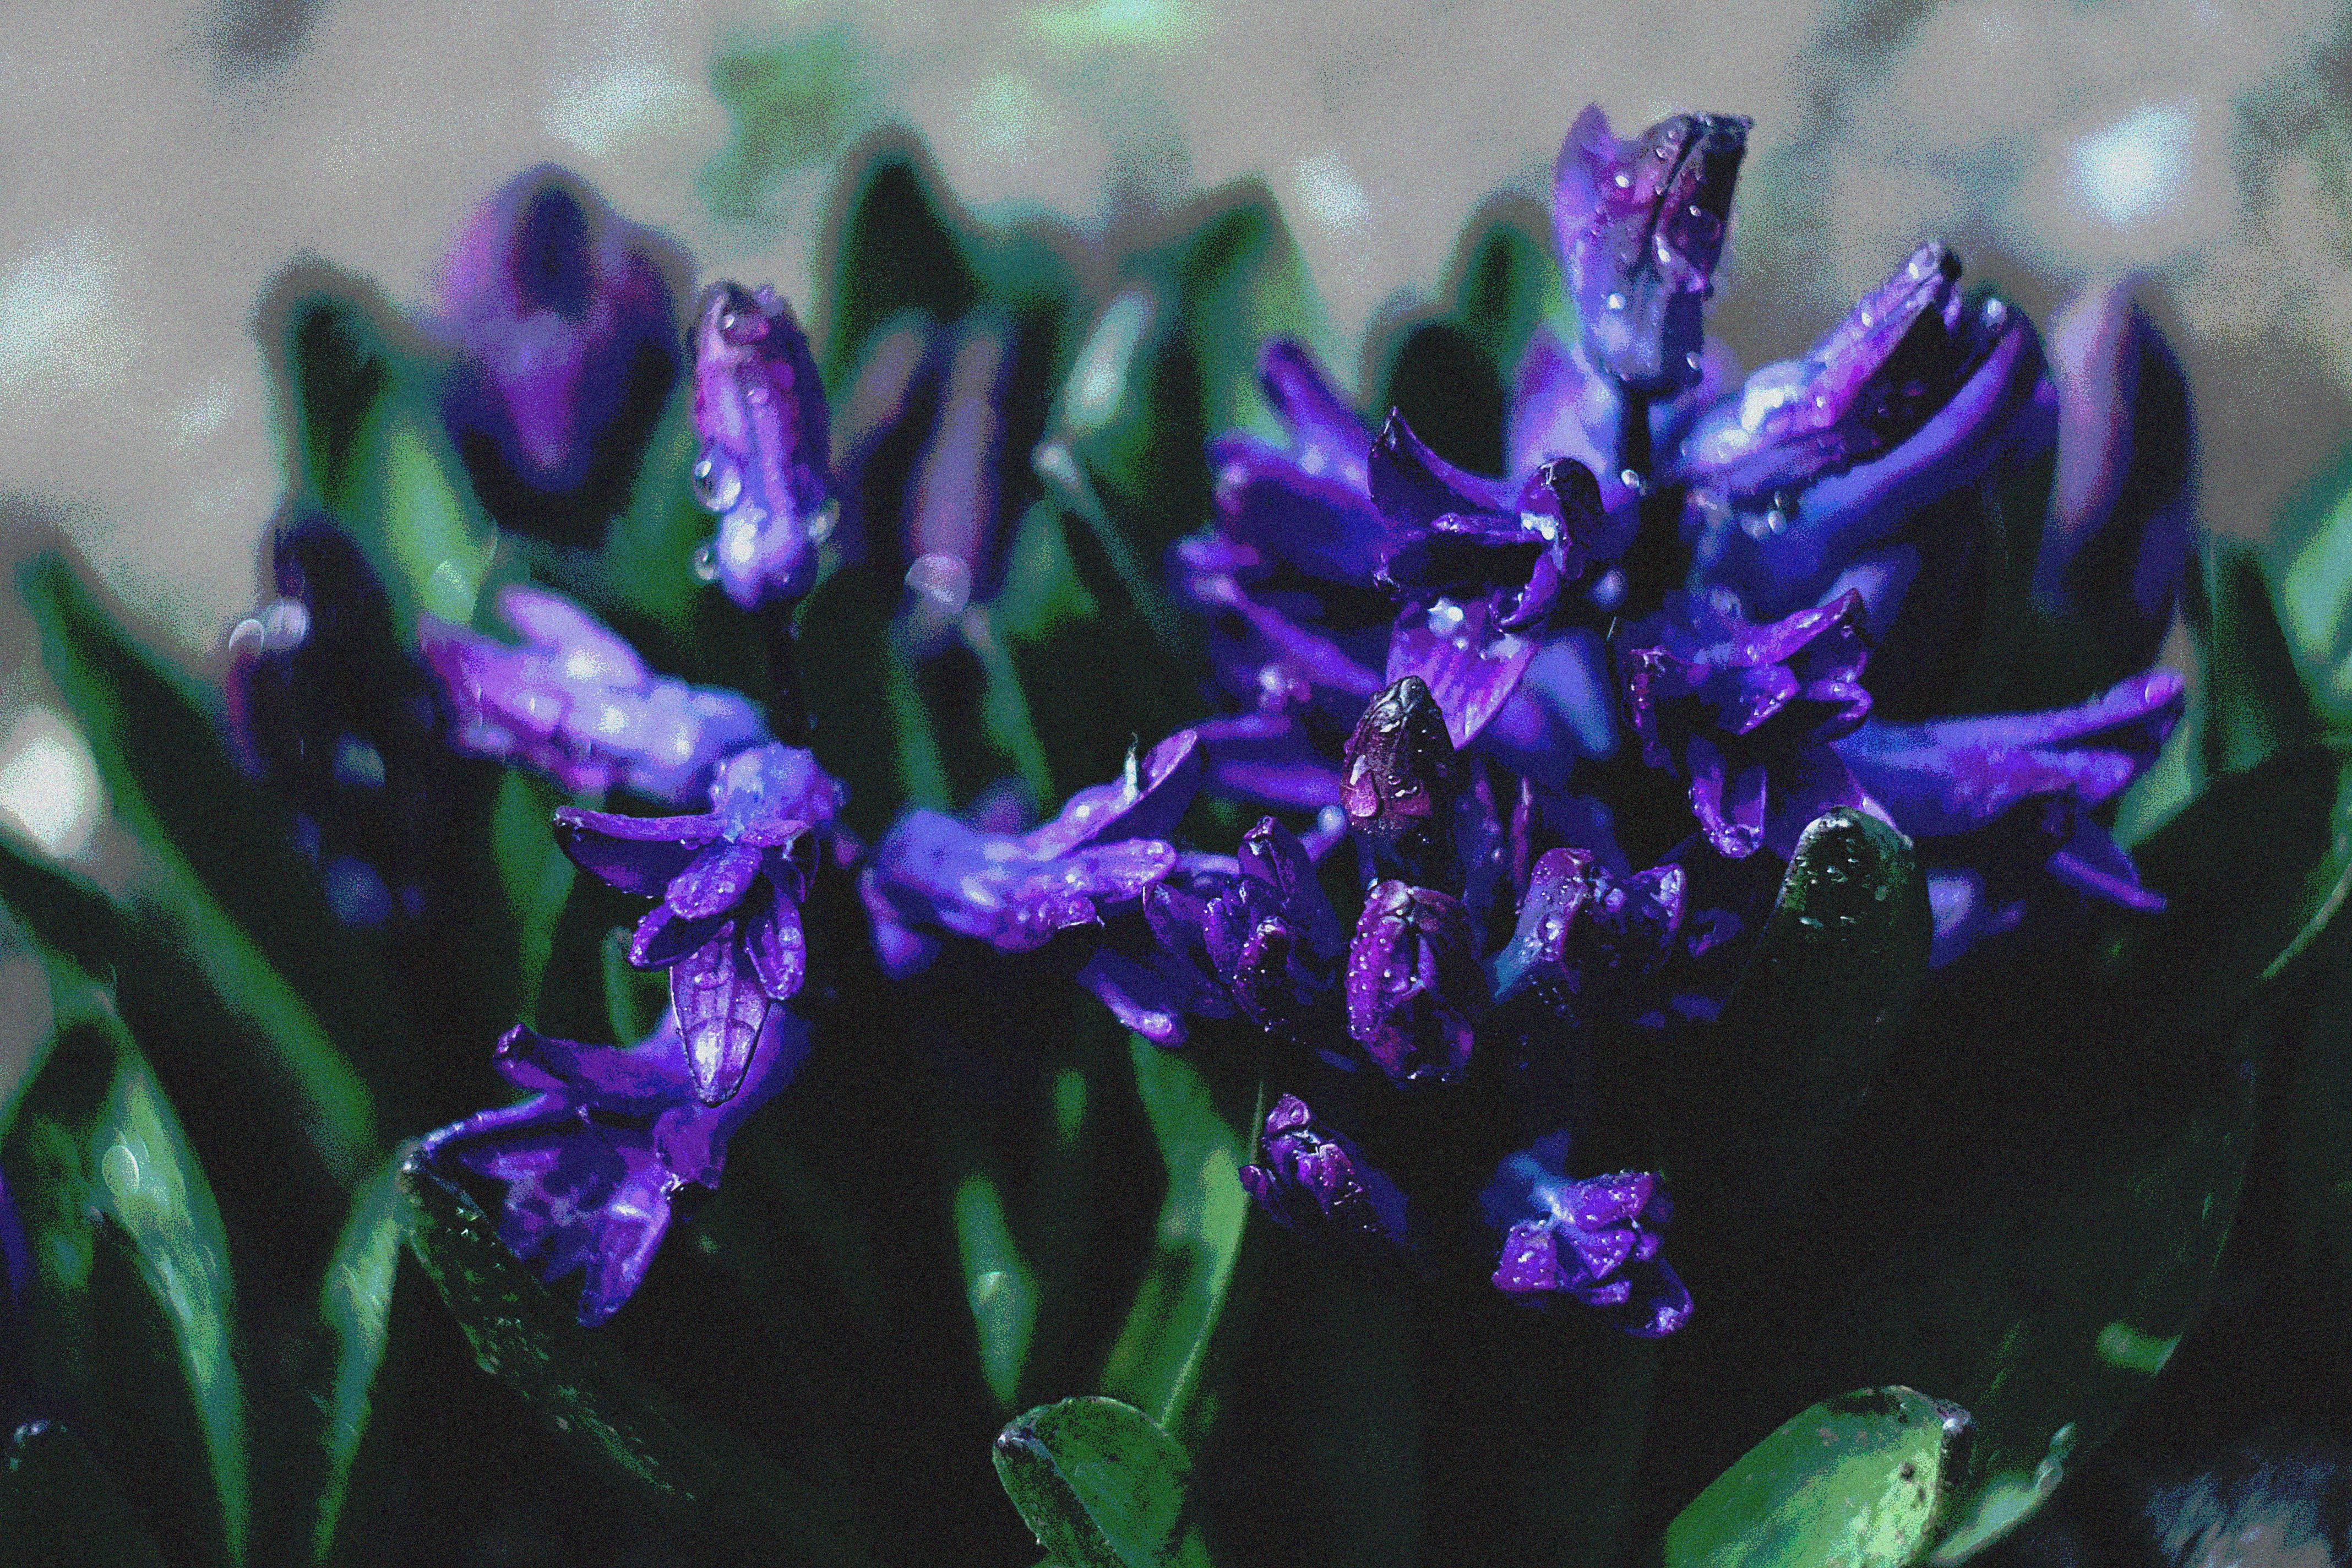
\includegraphics[width=1\textwidth]{flowers/flowers-72.png}
        \caption*{72\,\% (\num{26.3}\,MB)}
      \end{minipage}
    };

    \matrix [column sep=3.5cm] at ($(original.north)!0.5!(10mb.north) + (0,3.5cm)$) {
      \coordinate (a); & \coordinate (b); & \coordinate (c); & \coordinate (d); \\
    };

    \coordinate (spy-on) at (1.05cm,-0.55cm);

    \spy on ($(original.north) + (spy-on)$) in node[label=below:Original] at (a);
    \spy on ($(10mb.north) + (spy-on)$) in node[label=below:48\,\%] at (b);
    \spy on ($(20mb.north) + (spy-on)$) in node[label=below:60\,\%] at (c);
    \spy on ($(30mb.north) + (spy-on)$) in node[label=below:72\,\%] at (d);

  \end{tikzpicture}
  \caption{Blumen mit einer Größe von 2848 $\times$ 4272 Pixel.
    Gute Bildqualität bis zu 22\,MB versteckter
    Nachricht ($\bmax \approx \num{36.5}$\,MB).}
  \label{fig:example-flowers}
\end{figure}


\newpage

\noindent
Es kann beobachtet werden, dass
eine gute Bildqualität erreicht wird,
wenn die Grenze von vier Bitänderungen pro Farbkanal ($n = 4$) nicht überschritten wird.
Nachrichten mit einer Länge größer 50\,\% der maximalen Bildkapazität werden bis in die höheren
Bitstellen geschrieben und sind deshalb zunehmend schnell zu erkennen.
Nicht alle Bilder sind gleich gut geeignet um lange Nachrichten zu verstecken.
Änderungen bei \ref{fig:example-turtle} (Schildkröte) mit viel einfarbigen Hintergrund
lösen schneller einen sichtbaren Effekt aus als bei Bild \ref{fig:example-peppers}
(Paprika) oder \ref{fig:example-flowers} (Blumen), wo auch Nachrichten länger
50\,\% eher schwer zu erkennen sind. Bilder mit versteckten Nachrichten
sind empfindlich gegenüber Änderungen und sollten daher nicht als
Grafikformat mit verlustbehafteter Datenkompression gespeichert werden (z.\,B. JPEG).
Zusätzliche Informationen und der Quelltext zum Projekt
sind über den folgenden Link auf GitHub zu finden.
\footnote{https://github.com/jens-studienarbeit/image-data-hiding}

% Anhänge
\pagenumbering{Alph}
\printbibliography[title = Literaturverzeichnis]
\addcontentsline{toc}{chapter}{Literaturverzeichnis}
\printnoidxglossaries
\addcontentsline{toc}{chapter}{Glossar}
\end{document}